\documentclass[11pt, letterpaper,titlepage,oneside]{article}
%One inch margins
\usepackage[margin=1in]{geometry}
%Header/footer stuff
\usepackage{titlesec}
\usepackage{fancyhdr}
\fancyhf{}
\rfoot{\thepage}
\renewcommand{\headrulewidth}{0pt}
\pagestyle{fancy}
%paragraph indentation
\usepackage[parfill]{parskip}
\parskip = \baselineskip
\setlength{\parindent}{0in}
%Graphic Stuff
\usepackage{xcolor,graphicx}
\usepackage{float}
\usepackage{subcaption}
%Math tools
\usepackage{amsmath}
\usepackage{mathptmx}
\usepackage{lipsum}
%One and half spacing
\usepackage{setspace}
\onehalfspacing
%End one and a half spacing
%Algorithm
\usepackage{algorithm}
\usepackage{algorithmic}
\renewcommand{\arraystretch}{1}
% Caption Formatting
\usepackage{caption}
\captionsetup[figure]{labelsep=period}
\captionsetup[table]{labelsep=newline, justification=centering}
\renewcommand{\tablename}{TABLE}
\renewcommand{\thetable}{\Roman{table}}
\usepackage{fixltx2e}
%Title Page
\newcommand{\titles}{\LARGE \textbf{Partitioning Optimization for Massively Parallel Transport Sweeps on Unstructured Grids}}
\newcommand{\authors}{\normalsize Tarek Ghaddar \\ Chair: Dr. Jean Ragusa \\ Committee: Dr. Jim Morel, Dr. Marvin Adams, Dr. Nancy Amato}
\newcommand{\department}{\normalsize Nuclear Engineering Department}
\newcommand{\university}{\normalsize Texas A\&M University}
\newcommand{\locations}{\normalsize College Station, TX, 77843-3133}
%Script font
\usepackage[mathscr]{euscript}
\renewcommand{\thesection}{\Roman{section}.}
\renewcommand{\thesubsection}{\thesection\Alph{subsection}.}
\renewcommand{\thesubsubsection}{\thesection\Alph{subsection}.\arabic{subsubsection}}
%Include a pdf file
\usepackage{pdfpages}
%Using the .bib file
\usepackage[superscript,biblabel]{cite}
%Changing spacing in itemized lists
\usepackage{enumitem}
\setlist{nosep}

\newcommand{\tcr}[1]{\textcolor{red}{#1}}
\newcommand{\vr}{\vec{r}}
\newcommand{\vo}{\vec{\Omega}}

%%%%%%%%%%%%%%%%%%%%%%%%%%%%%%%%%%%%%%%%%%%%%%%%%%%%%%%%%%%%%%%%%%%%%
\begin{document}
%%%%%%%%%%%%%%%%%%%%%%%%%%%%%%%%%%%%%%%%%%%%%%%%%%%%%%%%%%%%%%%%%%%%%

\begin{titlepage}
\begin{center}
  \vspace*{3.81 cm}
  \titles\\
  \vspace*{4.445cm}
  \authors \\
  \vspace*{2.54cm} 
  \department \\
  \university \\
  \locations \\
\end{center}
\end{titlepage}


%%%%%%%%%%%%%%%%%%%%%%%%%%%%%%%%%%%%%%%%%%%%%%%%%%%%%%%%%%%%%%%%%%%%%
%%%%%%%%%%%%%%%%%%%%%%%%%%%%%%%%%%%%%%%%%%%%%%%%%%%%%%%%%%%%%%%%%%%%%
\section{Introduction}
%%%%%%%%%%%%%%%%%%%%%%%%%%%%%%%%%%%%%%%%%%%%%%%%%%%%%%%%%%%%%%%%%%%%%
%%%%%%%%%%%%%%%%%%%%%%%%%%%%%%%%%%%%%%%%%%%%%%%%%%%%%%%%%%%%%%%%%%%%%
Massively parallel transport sweeps have been shown to scale up to 750,000 cores on logically cartesian grids. However, structured meshes are somewhat limiting when  simulating more complex problems and experiments, requiring the use of unstructured meshes in transport sweeps. While unstructured meshes provide the ability to simulate realistic problems, they introduce some challenges like unbalanced partitions, which can increase the time to solution. To combat this, PDT, Texas A\&M University's massively parallel deterministic transport code, introduced two load balancing algorithms that rely on moving the spatial boundaries, or cut planes (cut lines in 2D), throughout the mesh in order to obtain a roughly equivalent amount of cells (and therefore work) per processor. However, this sacrifices the optimal partitioning scheme\cite{mpadams2013} in favor of balance. We propose a method that weighs ideal load balancing with the consequences to the transport sweep in order to achieve the best possible time to solution.

\subsection{Review of Neutron Transport and the Transport Sweep}

The steady-state neutron transport equation describes the behavior of neutrons in a medium and is given by Eq.~\eqref{continuous transport}:
\begin{equation}
\vo \cdot \vec \nabla \psi(\vr,E,\vo) +\Sigma_t(\vr,E) \psi(\vr,E,\vo)  =
\int_{0}^{\infty}dE' \int_{4\pi}d\Omega' \Sigma_s(\vr,E'\to E, \Omega'\to\Omega)\psi(\vr,E',\vo') 
+ S_{ext}(\vr,E,\vo) ,
\label{continuous transport}
\end{equation}
where $\vec{\Omega}\cdot \vec\nabla\psi$ is the leakage term and $\Sigma_t\psi$ is the total collision term (absorption, outscatter, and within group scattering). These represent the loss terms of the neutron transport equation. The right hand side of Eq.~\eqref{continuous transport} represents the gain terms, where $S_{ext}$ is the external source of neutrons and $\int_{0}^{\infty}dE'\int_{4\pi}d\Omega'\Sigma_s(E'\to E, \Omega'\to\Omega)\psi(\vr,E',\vo')$ is the inscatter term, which represents all neutrons scattering from energy $E'$ and direction $\vo'$ into $dE$ about energy $E$ and $d\Omega$ about direction $\vo$.

Without loss of generality for the problem at hand, we assume isotropic scattering for simplicity. The double differential scattering cross section, $\Sigma_s(E'\to E, \Omega'\to\Omega)$, has its angular dependence present in the integral, and it is divided by $4\pi$ to reflect isotropic behavior. This yields:
\begin{align}
\label{isotropic}
\vo \cdot \vec \nabla \psi(\vr,E,\vo) +\Sigma_t(\vr,E) \psi(\vr,E,\vo)  
& = \frac{1}{4\pi}\int_{0}^{\infty}dE' \Sigma_s(\vr,E'\to E) \int_{4\pi}d\Omega' \psi(\vr,E',\vo')  + S_{ext}(\vr,E,\vo) \nonumber \\
& = \frac{1}{4\pi}\int_{0}^{\infty}dE' \Sigma_s(\vr,E'\to E) \phi(\vr,E')  + S_{ext}(\vr,E,\vo) ,
\end{align}
where we have introduced the scalar flux as the integral of the angular flux:
\begin{equation}
\label{def_scalar_flux}
\phi(\vr,E') = \int_{4\pi}d\Omega' \psi(\vr,E',\vo').
\end{equation}
The next step to solving the transport equation is to discretize in energy, yielding Eq.~\eqref{multigroup} the multigroup transport equation:
\begin{equation}
\vo \cdot \vec \nabla \psi_g(\vr,\vo) +\Sigma_{t,g}(\vr) \psi_g(\vr,\vo) = \frac{1}{4\pi}\sum_{g^{\prime}}\Sigma_{s,g^{\prime}\to g}(\vr)\phi_{g^{\prime}}(\vr) + S_{ext,g}(\vr,\vo), \quad \text{for } 1 \le g \le G
\label{multigroup}
\end{equation}
where the multigroup transport equations now form a system of coupled equations. 

Next, we discretize in angle using the discrete ordinates method\cite{denovo}, whereby an angular quadrature $\left( \vo_m, w_m \right)_{1 \le m \le M}$ is used to solve the above equations along a given set of directions $\vo_m$:
\begin{equation}
\vo_m \cdot \vec \nabla \psi_{g,m}(\vr) +\Sigma_{t,g}(\vr) \psi_{g,m}(\vr)  = \frac{1}{4\pi}\sum_{g^{\prime}}\Sigma_{s,g^{\prime}\to g}(\vr)\phi_{g^{\prime}}(\vr) + S_{ext,g,m}(\vr),
\label{angle}
\end{equation}
where the subscript $m$ is introduced to describe the angular flux in direction $m$. The subscript is not added to our inscatter term because of the isotropic scattering assumption and because the scalar flux does not depend on angle. However, in order to evaluate the scalar flux, we employ the angular weights $w_m$ and the angular flux solutions
$\psi_m$ to numerically perform the angular integration:
\begin{equation}
\label{def_scalar_flux_2}
\phi_g(\vr) \approx \sum_{m=1}^{m=M} w_m \psi_{g,m}(\vr).
\end{equation}

At this point, it is clear that we are solving a sequence of transport equations, solving for one group and direction at a time. Therefore, all transport equations are of the following form:
\begin{equation}
\vo_m \cdot \vec \nabla \psi_{m}(\vr) +\Sigma_{t}(\vr) \psi_{m}(\vr)  = \frac{1}{4\pi}\Sigma_{s}(\vr)\phi(\vr) + q^{ext+inscat}_m(\vr) = q_m(\vr),
\end{equation}
where the group index is omitted for brevity.

In order to obtain the solution for this discrete form of the transport equation, an iterative process, source iteration, is introduced. This is shown by a simplified transport equation Eq. ~\eqref{iteration}:
\begin{equation}
\vo_m \cdot \vec\nabla \psi_m^{(l+1)}(\vr) + \Sigma_t \psi_m^{(l+1)}(\vr) = q_m^{(l)}(\vr),
\label{iteration}
\end{equation}
where the right hand side terms of Eq.~\eqref{angle} have been combined into one general source term, $q_m$. The angular flux of iteration $(l+1)$ is calculated using the $(l^{th})$ value of the scalar flux.

After the angular and energy dependence have been accounted for, Eq.~\eqref{iteration} must be discretized in space as well. This is done by meshing the domain and utilizing one of three popular discretization techniques: finite difference\cite{fd}, finite volume\cite{fd}, or discontinuous finite element\cite{Reed}, allowing one cell at a time to be solved. The solution across a cell interface is connected based on an upwind approach, where face outflow radiation becomes face inflow radiation for the downwind cells. Figure \ref{sweeps} shows the sweep ordering for a given direction on both a structured and unstructured mesh.

\noindent\begin{minipage}{\textwidth}
\centering
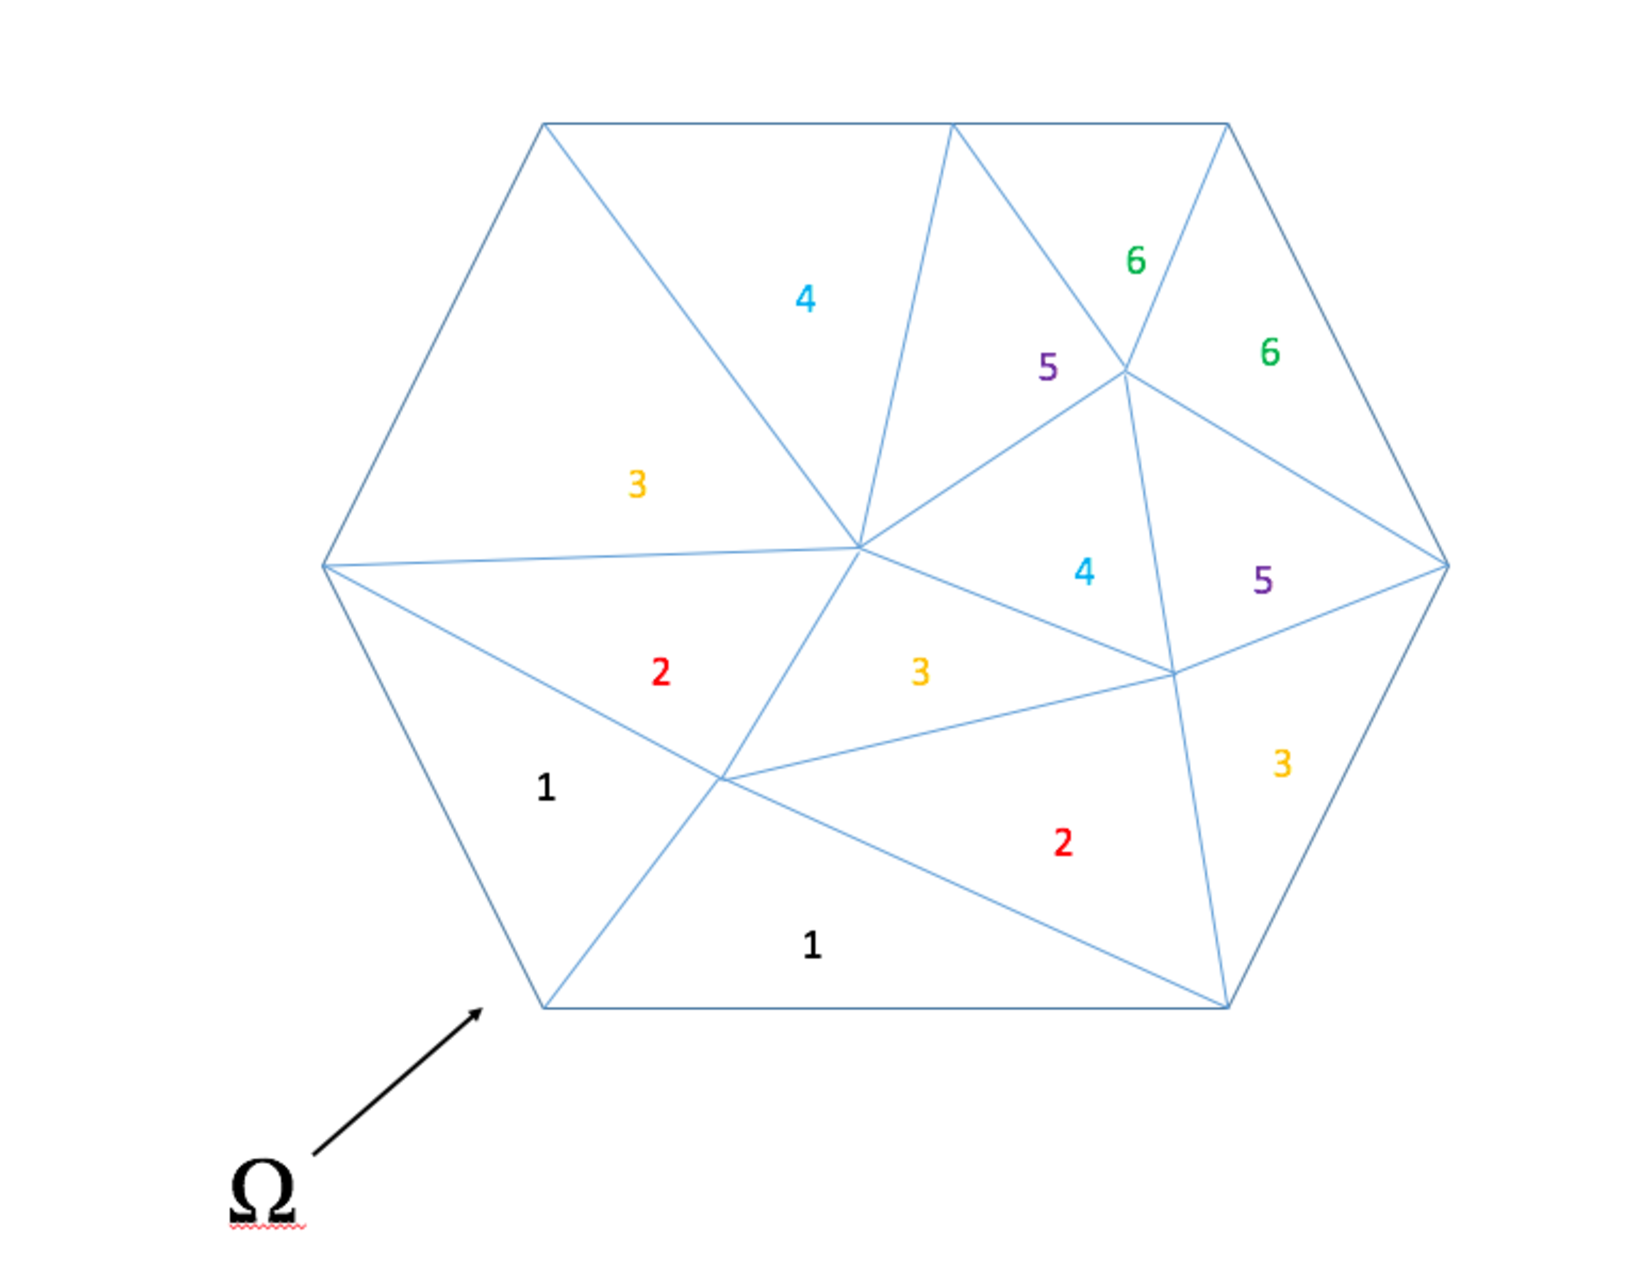
\includegraphics[scale = 0.27]{../figures/UnstructureMesh.pdf}
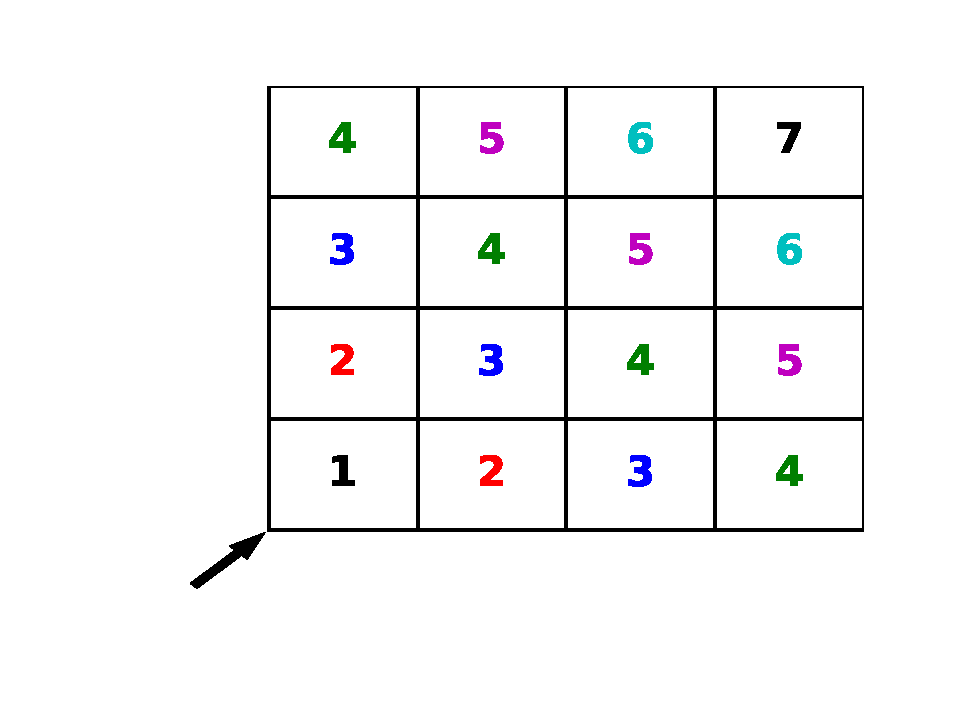
\includegraphics[scale = 0.27]{../figures/StructuredMesh.pdf}
\captionof{figure}{A demonstration of a sweep on a structured and unstructured mesh. }
\label{sweeps}
\end{minipage}
\smallskip

The number in each cell represents the order in which the cells are solved. All cells must receive the solution downwind from them before solving for their own solution. This dependency can be represented and stored as a task dependence graph, shown in Fig. \ref{tdg}.

\noindent\begin{minipage}{\textwidth}
\centering
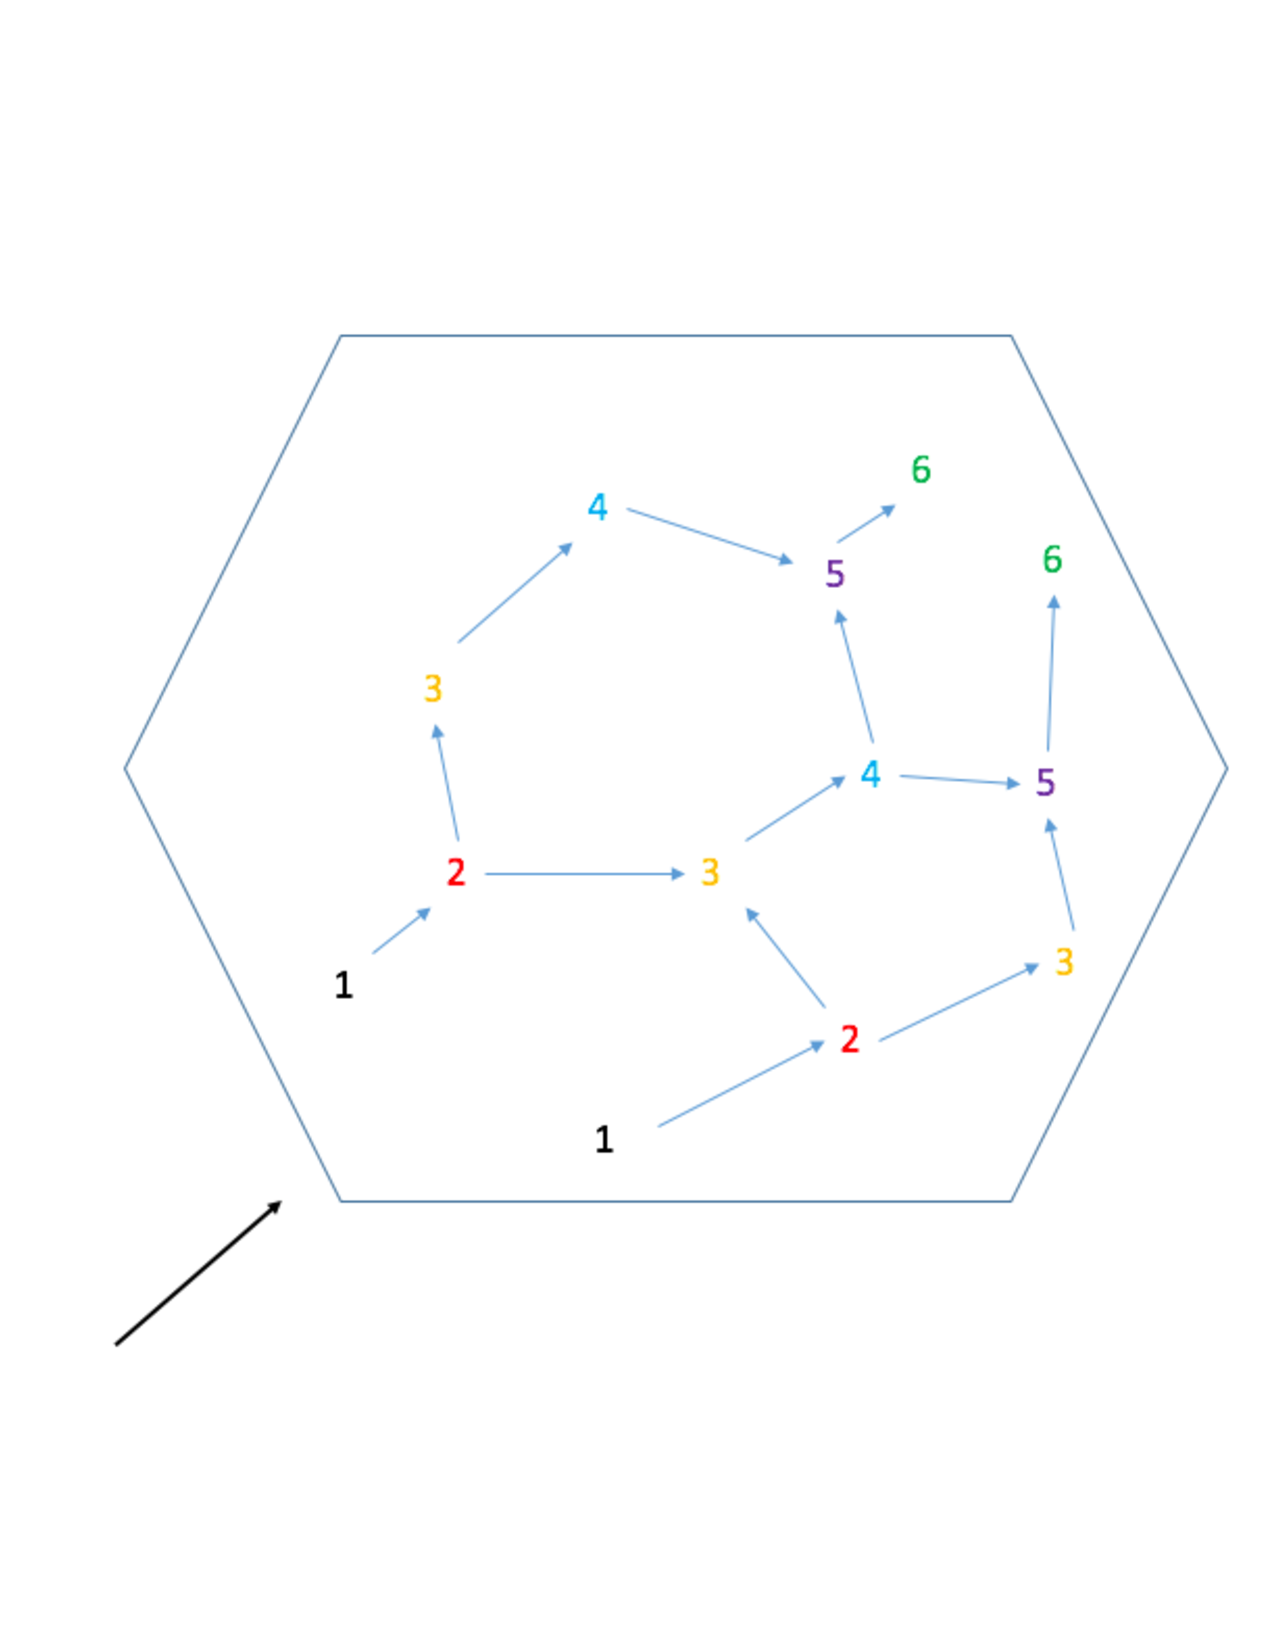
\includegraphics[scale = 0.35]{../figures/tdg.pdf}
\captionof{figure}{A task dependence graph of the unstructured mesh example in Fig. \ref{sweeps}.}
\label{tdg}
\end{minipage}
\smallskip

The concepts presented in this introduction are used by PDT, Texas A\&M University's massively parallel deterministic transport code. It is capable of multi-group simulations and employs discrete ordinates for angular discretization. PDT features steady-state, time-dependent, criticality, and depletion simulations, and solves the transport equation for neutron, thermal, gamma, coupled neutron-gamma, electron, and coupled electron-photon radiation. PDT has been shown to scale on logically Cartesian grids out to \tcr{750,000} cores. Logically Cartesian grids contain regular convex grid units that allow for vertex motion inside them, in order to conform to curved shapes. Much of the work completed and proposed in this document uses PDT or was developed in PDT. 
%%%%%%%%%%%%%%%%%%%%%%%%%%%%%%%%%%%%%%%%%%
%%%%%%%%%%%%%%%%%%%%%%%%%%%%%%%%%%%%%%%%%%
\section{Review of Parallel Transport Sweeps}
%%%%%%%%%%%%%%%%%%%%%%%%%%%%%%%%%%%%%%%%%%
%%%%%%%%%%%%%%%%%%%%%%%%%%%%%%%%%%%%%%%%%%

As mentioned in the previous section, a transport sweep is set up by overlaying a domain with a finite element mesh. The sweep then solves the transport equation cell by cell using a discontinuous finite element approach. A task dependence graph gives the order in which cells are solved, as shown in Fig. \ref{tdg}. The transport sweep can be solved in parallel in order to obtain the solution faster, as well as distribute the problem across many processors for memory intensive cases. In PDT, a transport sweep can be performed on a structured Cartesian or arbitrary polyhedral mesh. Sweeping on an unstructured mesh presents two big challenges: maintaining sweep efficiency on a massively parallel scale and keeping non-concave sub-domains to avoid cycles. PDT has already proven the ability to perform massively parallel transport sweeps on structured meshes. As part of previous efforts in PDT, researchers have come to outline three important properties for parallel sweeps. 

A parallel sweep algorithm is defined by three properties\cite{mpadams2013} :
\begin{itemize}
\item partitioning: dividing the domain among available processors,
\item aggregation: grouping cells, directions, and energy groups into tasks,
\item scheduling: choosing which task to execute if more than one is available.
\end{itemize}

The basic concepts of parallel transport sweeps, partitioning, aggregation, and scheduling, are most easily described in the context of a structured transport sweep that takes place on a Cartesian mesh. Furthermore, the work proposed utilizes aspects of the structured transport sweep.

In a regular grid, we have the  number of cells in each Cartesian direction: $N_x, N_y, N_z$. These cells are aggregated into ``cellsets'', using aggregation factors $A_x, A_y, A_z$. If $M$ is the number of angular directions per octant, $G$ is the total number of energy groups, and $N$ is the total number of cells, then the total fine grain work units is $8MGN$. The factor of 8 is present as $M$ directions are swept for all 8 octants of the domain. The finest grain work unit is the calculation of a single direction and energy group's unknowns in a single cell, or $\psi_{m,g}$ for a single cell.

Fine grain work units are aggregated into coarser-grained units called \textit{tasks}. A few terms are defined that describe how each variable is aggregated.
\begin{itemize}
\item $A_x = \frac{N_x}{P_x}$, where $N_x$ is the number of cells in $x$ and $P_x$ is the number of processors in $x$
\item $A_y = \frac{N_y}{P_y}$, where $N_y$ is the number of cells in $y$ and $P_y$ is the number of processors in $y$
\item $A_z$ = a selectable number of z-planes of $A_x A_y$ cells.
\item $N_g = \frac{G}{A_g}$
\item $N_m = \frac{M}{A_m}$
\item $N_k = \frac{N_z}{P_z A_z}$
\item $N_k A_x A_y A_z = \frac{N_x N_y N_z}{P_x P_y P_z}$
\end{itemize}

It follows that each process owns $N_k$ cell-sets (each of which is $A_z$ planes of $A_x A_y$ cells), $8N_m$ direction-sets, and $N_g$ group-sets for a total of $8N_m N_g N_k$ tasks.

One task contains $A_x A_y A_z$ cells, $A_m$ directions, and $A_g$ groups. Equivalently, a task is the computation of one cellset, one groupset, and one angleset, with the completion of one task defined as a stage.  The stage is particularly important when assessing sweeps against analytical performance models. 

Equation ~\eqref{paralleleff} approximately defines parallel sweep efficiency. This can be calculated for specific machinery and partitioning parameters by substituting in values calculated using Eqs.~\eqref{nfill},~\eqref{nidle}, and ~\eqref{ntasks}.
\begin{equation}\label{paralleleff}
\begin{split}
\epsilon &= \frac{T_{\text{task}} N_{\text{tasks}}}{[N_{\text{stages}}] [T_{\text{task}} + T_{\text{comm}}]} \\
            &=\frac{1}{[1+\frac{N_{\text{idle}}}{N_{\text{tasks}}}][1 + \frac{T_{\text{comm}}}{T_{\text{task}}}]}
\end{split}
\end{equation}

Equations ~\eqref{Tcomm} and ~\eqref{Ttask} show how $T_{\text{comm}}$ and $T_{\text{task}}$ are calculated:
\begin{equation}
T_{\text{comm}} = M_L T_{\text{latency}} + T_{\text{byte}} N_{\text{bytes}}
\label{Tcomm}
\end{equation}
\begin{equation}
T_{\text{task}} = A_x A_y A_z A_m A_g T_{\text{grind}}
\label{Ttask}
\end{equation}
where $T_{\text{latency}}$ is the message latency time, $T_{\text{byte}}$ is the time required to send one byte of message, $N_{\text{bytes}}$ is the total number of bytes of information that a processor must communicate to its downstream neighbors at each stage, and $T_{\text{grind}}$ is the time it takes to compute a single cell, direction, and energy group. $M_L$ is a latency parameter that is used to explore performance as a function of increased or decreased latency. If a high value of $M_L$ is necessary for the model to match computational results, improvements should be made in code implementation.

\subsection{KBA Partitioning for Structured Grids}

Several parallel transport sweep codes use KBA partitioning in their sweeping, such as Denovo \cite{denovo} and PARTISN \cite{partisn}. The KBA partitioning scheme and algorithm was developed by Koch, Baker, and Alcouffe \cite{partisn}.

The KBA algorithm traditionally chooses $P_z = 1, A_m = 1, G = A_g = 1, A_x = N_x/P_x, A_y = N_y/P_y$, with $A_z$ being the selectable number of z-planes to be aggregated into each task. With $N_k = N_z/A_z$, each processor performs $N_{\text{tasks}} = 8MN_k$ tasks. With the KBA algorithm, $2MN_k$ tasks are pipelined from a given corner of the 2D processor layout. The far corner processor remains idle for the first $P_x + P_y - 2 $ stages, which means that an octant-pair (or quadrant) sweep completes in $2MN_k + P_x + P_y - 2$ stages. If an octant-pair sweep does not begin until the previous pair's finishes, the full sweep requires $8MN_k + 4(P_x+P_y-2)$ stages, which means the KBA parallel efficiency is:
\begin{equation}
\varepsilon_{KBA} = \frac{1}{[1+\frac{4(P_x+P_y-2)}{8MN_k}][1+\frac{T_{\text{comm}}}{T_{\text{task}}}]}
\label{eKBA}
\end{equation}

%%%%%%%%%%%%%%%%%%%%%%%%%%%%%%%%%%%%%%%%%%%%%%%%%%%%%%%%%%%%%%%%%%%%%
\subsection{The Structured Transport Sweep in PDT}
%%%%%%%%%%%%%%%%%%%%%%%%%%%%%%%%%%%%%%%%%%%%%%%%%%%%%%%%%%%%%%%%%%%%%
The minimum possible number of stages for given partitioning parameters $P_i$ and $A_j$ is $2 N_{\text{fill}}+N_{\text{tasks}}$. $N_{\text{fill}}$ is both the minimum number of stages before a sweepfront can reach the center-most processors and the number needed to finish a direction's sweep after the center-most processors have finished. Equations~\eqref{nfill}, ~\eqref{nidle}, and~\eqref{ntasks} define $N_{\text{fill}}$, $N_{\text{idle}}$, and $N_{\text{tasks}}$:
\begin{equation}
N_{\text{fill}} = \frac{P_x + \delta_x}{2} - 1 + \frac{P_y + \delta_y}{2} - 1 + N_k (\frac{P_z + \delta_z}{2} - 1)
\label{nfill}
\end{equation}
\begin{equation}
N_{\text{idle}} = 2 N_{\text{fill}}
\label{nidle}
\end{equation}
\begin{equation}
N_{\text{tasks}} = 8 N_m N_g N_k
\label{ntasks}
\end{equation}
where $\delta_u$ is 1 for $P_u$ odd, and 0 for $P_u$ even.

Figure \ref{partitioning} shows three different partitioning schemes used in transport sweeps, KBA (which is defined in the previous section), volumetric non-overloaded, and volumetric overloaded. Volumetric non-overloaded requires that all cells owned by a processor are contiguous, where as volumetric non-overloaded partitioning does not have this restriction.  

\noindent\begin{minipage}{\textwidth}
\centering
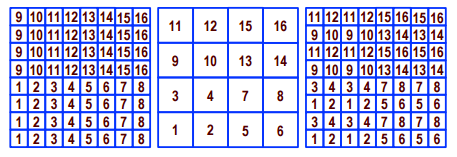
\includegraphics[scale = 1]{../figures/Partitioning.PNG}
\captionof{figure}{Three different partitioning schemes in 2D, from left to right: KBA, volumetric non-overloaded, and volumetric overloaded.}
\label{partitioning}
\end{minipage}

The overloaded volumetric partitioning proceeds as follows:

\begin{enumerate}
\item In a 2D (3D) domain, cellsets are divided into 4 (8) spatial quadrants (octants), with an equal number of cellsets in each  SQO (SQO is defined as a spatial quadrant or octant).
\item Assign 1/4 of the processors (1/8) in 3D to each SQO. 
\item Choose the individual overload factors $\omega_x, \omega_y, \text{and } \omega_z$ and individual processor counts $P_x, P_y, \text{and }P_z$, such that $\omega_x \omega_y \omega_z = \omega_r$ and $P_x P_y P_z = P$, with all $P_u$ even. $\omega_u$ is defined as the number of cellsets assigned to each $P_u$.
\item An array of $\omega_x\cdot\omega_y\cdot\omega_z$ ``tiles'' in each SQO. Each tile is an array of $1/2 P_x \cdot 1/2 P_y \cdot 1/2 P_z$ cellsets. These cellsets are mapped one-to-one to the $1/2 P_x \cdot 1/2 P_y \cdot 1/2 P_z$ processors assigned to the SQO, using the same mapping in each tile.
\end{enumerate}
Each tile has a logically identical layout of cellsets, and each processor owns exactly one cellset in each tile in its SQO. This makes each processor responsible for $\omega_r$ cellsets.

In order to properly outline the optimal scheduling rules, the variables $X,Y, \text{and } Z$ are defined as $P_u/2$ for each respective direction $u = x,y,z$. This splits up the processor layout into octants, where each processor has an index $(i,j,k)$ determining where it is in the layout. Tiles are also indexed and referred to in the same way with the notation $T(i,j,k)$. 

The optimal scheduling algorithm rules are as follows:
\begin{enumerate}
\item If $i \leq X$, then tasks with $\Omega_x > 0$ have priority, while for $i > X$, tasks with $\Omega_x < 0$ have priority.
\item If multiple ready tasks have the same sign on $\Omega_x$, apply rule 1 to $j,Y,\Omega_y$.
\item If multiple ready tasks have the same sign on $\Omega_x$ and $\Omega_y$, apply rule 1 to $k,Z, \Omega_z$. 
\item If multiple tasks are ready in the same octant, then priority goes to the cellset for which the priority octant has greatest downstream depth.
\item If multiple ready tasks are in the same octant and have the same downstream depth of graph in $x$, then priority goes to the cellset for which the priority octant has greatest downstream depth of graph in $y$.
\item If multiple ready tasks are in the same octant and have the same downstream depth of graph in $x$ and $y$, then priority goes to the cellset for which priority octant has greatest depth of graph in $z$.
\end{enumerate}
This ensures that each SQO orders the octants: the one it can start right away ($A$), three that have one sign difference from $A (B,C,$ and $D)$, three that have two sign differences ($\bar D, \bar C, \bar B$), and one in opposition to its primary ($\bar A$). For example, if octant $A$ is octant $(+x, +y, +z)$, then it's secondary octants (only one sign change at a time) would be octants $(-x, +y, +z)$, $(+x,-y,+z)$ and $(+x,+y,-z)$.

There are three constraints in order to achieve the optimal stage count. In these constraints, $M = \omega_g \omega_m/8$, which is the number of tasks per octant per cellset.
\begin{enumerate}
\item $ M \geq 2(Z-1)$
\item $\omega_z M \geq 2(Y-1)$
\item If $\omega_x > 1$, then $\omega_y \omega_z M \geq X$
\end{enumerate}
Constraint 1 ensures that there is no idle time between a processor finishing an octant's work in one tile and beginning that octant's work on the next tile in the same tile-column; processor $P(1,Y,1)$ finishing its tile $T(1,\omega_y,1)$ octant $C$ work and beginning its octant $B$ work; processor $P(X,1,1)$ finishing its tile $T(\omega_x,1,1)$ octant $D$ work and beginning its octant $B$ work. Constraint 2 ensures that there is no idle time time between a processor finishing an octant's work for one $z$ column of tiles and beginning that octant's work on the next column; processor $P(X,1,1)$ finishing its tile $T(\omega_x,1,1)$ octant D work available to it and beginning its octant $C$ work. Constraint 3 ensures that there is no idle time between a processor finishing an octant's work for one $yz$ plane of tiles and beginning that octant's work in the next plane.

As a result of these constraints, there is no idle time for a variety of situtations. At large processor counts, the product $\omega_m \omega_g$ must be large, which requires $N_m N_g$ be large. This means that a weak scaling series refined only in space, but only coarsely refined in angle and energy, will eventually fail the constraints.

The optimal efficiency formula changes slightly from the KBA and hybrid KBA partitioning method in order to account for the overload factors. The only change is in the $\frac{N_{idle}}{N_{tasks}}$ term, as shown in Eq. ~\eqref{overloadpartitioning}. 
\begin{equation}
\varepsilon_{opt} = \frac{1}{[1+\frac{P_x+P_y+P_z-6}{\omega_g \omega_m \omega_r}][1+\frac{T_{\text{comm}}}{T_{\text{task}}}]}
\label{overloadpartitioning}
\end{equation}

%%%%%%%%%%%%%%%%%%%%%%%%%%%%%%%%%%%%%%%%%%%%%%
\subsection{Extension of Parallel Transport by Pautz and Bailey}
%%%%%%%%%%%%%%%%%%%%%%%%%%%%%%%%%%%%%%%%%%%%%%%
Pautz and Bailey\cite{PautzBailey} extended the work of Adams et al with overloaded unstructured partitioning. From their article, Figs. 3 through 9\cite{PautzBailey} showcase the different partitioning schemes used.  Weak scaling results were generated using the SCEPTRE transport code\cite{sceptre}. From these studies, Pautz and Bailey made the following observations:
\begin{enumerate}
	\item At low levels of parallelism, increased amounts of overloading lead to increased run times.
	\item With higher core counts, improvements are seen when the amount of overloading is increased.
	\item Results from unstructured and structured overloading are comparable. 
	\item Hybrid KBA often, but not always, outperformed overloaded partitions. If sufficient overloading was used, the results were comparable.
	\item Results in two dimensions are more pronounced that in three dimensions.
\end{enumerate}


%%%%%%%%%%%%%%%%%%%%%%%%%%%%%%%%%%%%%%%%%%
\subsection{The Unstructured Transport Sweep}
%%%%%%%%%%%%%%%%%%%%%%%%%%%%%%%%%%%%%%%%%%
In an unstructured mesh, the number of cells cannot be described in the same way as an unstructured mesh. In PDT specifically we initially subdivide the domain into subsets, which are just rectangular subdomains. Within each subset, an unstructured mesh is created. This creates a pseudo-regular grid. These subsets become the $N_x, N_y, N_z$ equivalent for an unstructured mesh. The spatial aggregation in a PDT unstructured mesh is done by aggregating subsets into cellsets. 

While the structured PDT transport sweep has scaled well out to 750,000 cores, similar levels of parallel scaling have not been achieved using unstructured sweeps yet. Pautz proposed a list scheduling algorithm has been constructed for modest levels of parallelism (up to 126 processors)\cite{Pautz} .

There are three requirements for a sweep scheduling algorithm to have. First, the algorithm should have low complexity, since millions of individual tasks are swept over in a typical problem. Second, the algorithm should schedule on a set of processors that is small in comparison to the number of tasks in the sweep graph. Last, the algorithm should distribute work in the spatial dimension only, so that there is no need to communicate during the calculation of the scattering source. 

Here is the pseudocode for the algorithm:

\begin{verbatim}
Assign priorities to every cell-angle pair
Place all initially ready tasks in priority queue
While (uncompleted tasks)
    For i=1,maxCellsPerStep
       Perform task at top of priority queue
       Place new on-processor tasks in queue
    Send new partition boundary data
    Receive new partition boundary data
    Place new tasks in queue 
\end{verbatim}

An important part of the algorithm above is the assigning priorities to tasks. Specialized prioritization heuristics generate partition boundary data as rapidly as possible in order to minimize the processor idle time. 

Nearly linear speedups were obtained on up to 126 processors. Further work is being done for scaling to thousands of processors. 

\subsubsection{Cycle Detection}

A cycle is a loop in a directed graph and they can occur commonly in unstructured meshes. However, they do not exist in 2D triangular extruded problems (PDT's primary unstructured meshing capability) and because our domain partitioning is convex, arbitrary degenerate polygons appearing on subdomain boundaries will not produce cycles. However, when using an Cubit/OpenFOAM generated mesh, we get cycles when aggregating angles. Because of this, cycle detection is discussed for completeness. 

Cycles can cause hang time in the problem, as a processor will wait for a message that might will never come. This means that the computation for one or more elements will never be completed. The solution to this is to ``break'' any cycles that exist by removing an edge of the task dependence graph (TDG). Old flux information is used on a particular element face in the domain. Most of the time, the edge removed is oriented obliquely with respect to the radiation direction. 

Algorithms for finding cycles are called \textit{cycle detection} algorithms. This must be done efficiently in parallel, both because the task dependence graph is distributed and because the finite element grid may be deforming every timestep and changing the associated TDG.

Cycle detection utilizes two operations: trim and mark. Trimming identifies and discards elements which are not in cycles. At the beginning of cycle detection, graphs are trimmed in the downwind direction, then the remaining graphs are trimmed in the upwind direction. A pivot vertex is then selected in each graph. Graph vertices are then marked as upwind, downwind, or unmarked. Then, if any vertices are both upwind and downwind, the cycle is these vertices plus the pivot vertex. An edge is removed between 2 cycle vertices, and 4 new graphs are created: a new cycle, the upwind vertices without the cycle, the downwind vertices without the cycle, and a set of unmarked vertices. This recursively continues until all cycles are eliminated.

\section{Review of Unstructured Meshing in PDT}

The capability for PDT to generate and run on an unstructured mesh is important because it allows us to run problems without having to conform our mesh to the problem. The idea is to have a logically Cartesian grid (creating orthogonal ``subsets") with an unstructured mesh inside each subset. These logically Cartesian subdomains are obtained using cut planes in 3D and cut lines in 2D. Figure \ref{grid} demonstrates this functionality, with the first two subsets meshed using the Triangle Mesh Generator\cite{triangle}, a 2D mesh generator. 

\noindent\begin{minipage}{\textwidth}
\centering
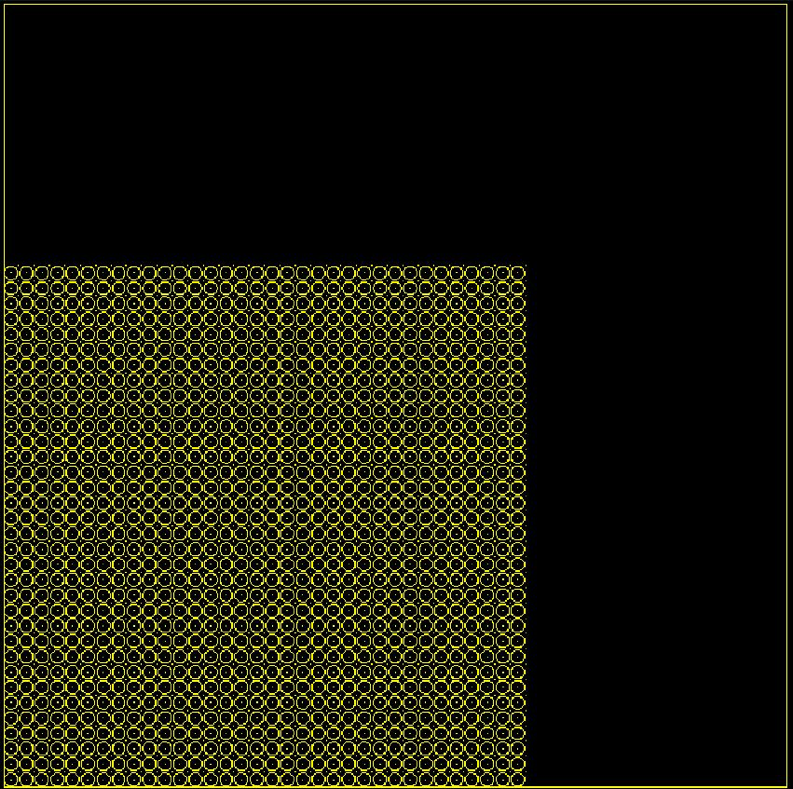
\includegraphics[scale = 0.5]{../figures/lattice.png}
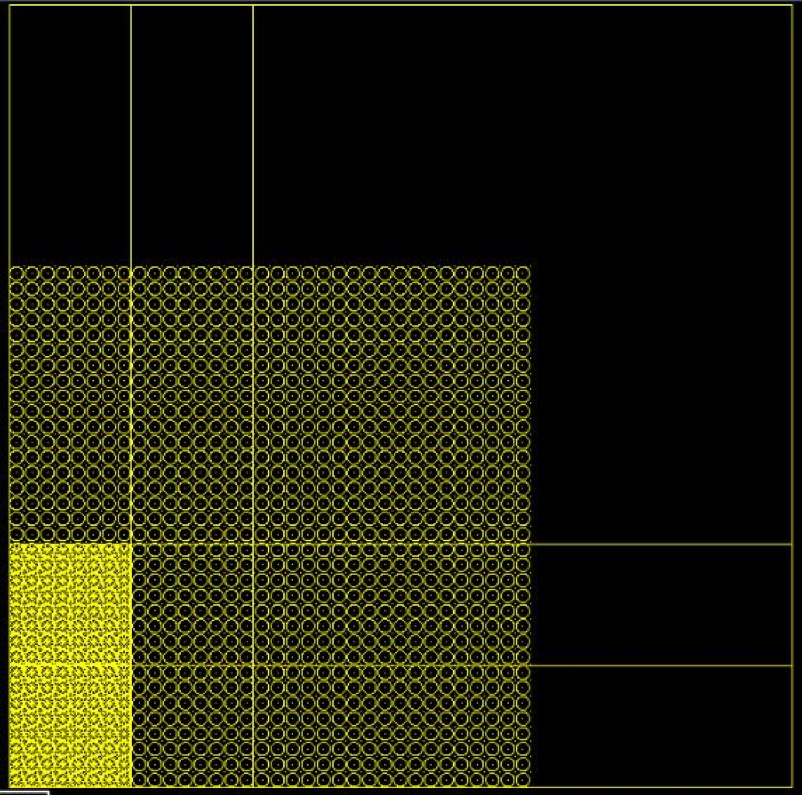
\includegraphics[scale = 0.5]{../figures/subsetlattice.png}
\captionof{figure}{A PSLG describing a fuel lattice, and with a orthogonal ``subset" grid imposed on on the PSLG.}
\label{grid}
\end{minipage}

This orthogonal grid is superimposed and each subset is meshed in parallel.  Subsets are now the base structured unit when calculating our parallel efficiency. Discontinuities along the boundary are fixed by ``stitching'' hanging nodes, creating degenerate polygons along subset boundaries. Because PDT's spatial discretization employs Piece-Wise Linear Discontinuous (PWLD) finite element basis functions, there is no problem solving on degenerate polygons. 

\subsection{Triangular Meshes in PDT}

When using the Triangle unstructured meshing capability in PDT, the input geometry is described by a Planar Straight Line Graph (PSLG). After superimposing the orthogonal grid, a PSLG is created for each subset, and meshed.  Because the input's and each subset's PSLG must be described and meshed in 2D, the mesh can be extruded in the $z$ dimension in order to give us the capability to run on 3D problems. Obviously, this is not as good as a unstructured tetrahedral mesh, but for many problems, it is a great capability to have. 

\subsection{OpenFOAM Meshes in PDT}

PDT has recently acquired the ability to read in OpenFOAM meshes and sweep on them. Rick Vega (a Texas A\&M graduate under Marvin Adams) adapted the load balancing by dimension algorithm used in PDT into a fully 3D case (discussed later). His code accepts a fluent mesh file, load balances it, and dumps the balanced mesh in OpenFOAM format. PDT then reads in the OpenFOAM formatted file and sweeps on that mesh. This approach has major advantages to the Triangle approach, because it allows a user with an existing mesh (generated via Cubit, Star CCM, TetGen, etc.) to simply save the mesh as a fluent file and have PDT read it in and sweep on it. Figures \ref{comparison}, \ref{comparison_slice}, and \ref{comparison_slice_zoom} show the differences in the two above approaches for the IM1C experiment run at Texas A\&M University.

\begin{figure}[H]
\centering
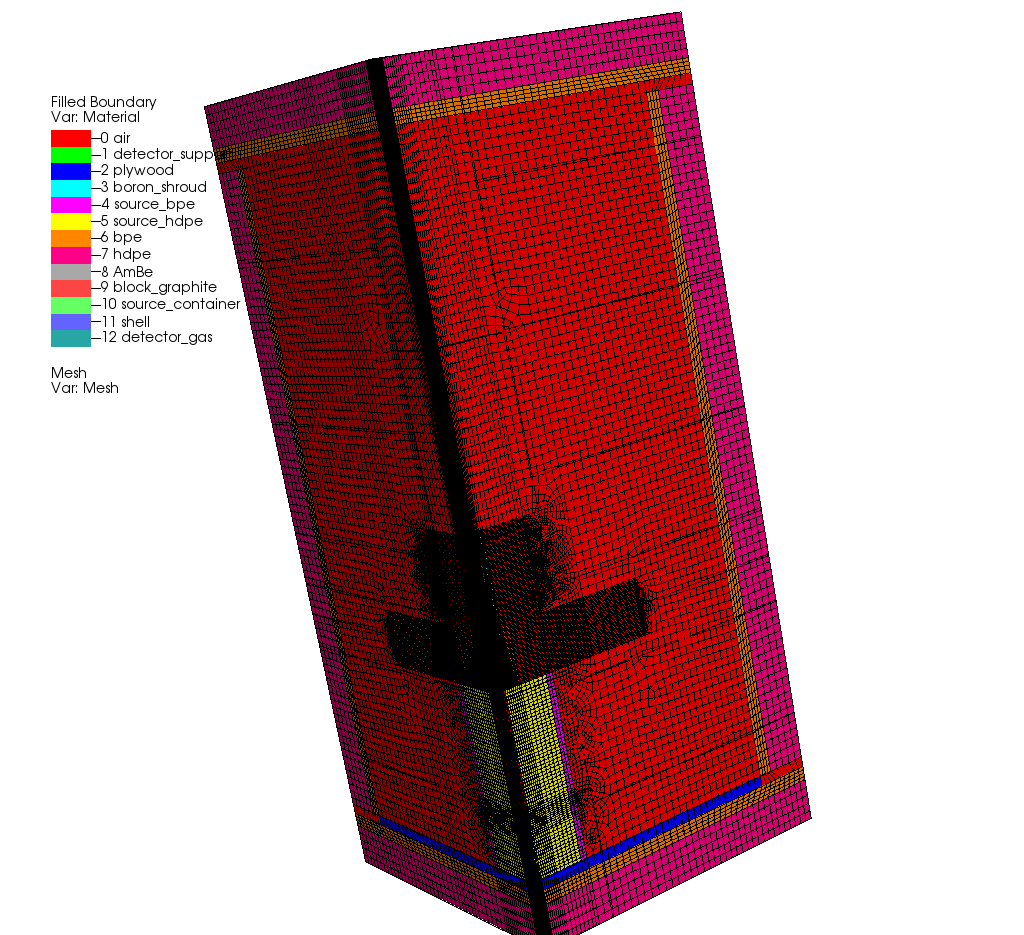
\includegraphics[scale=0.17]{../figures/im1_228.png}
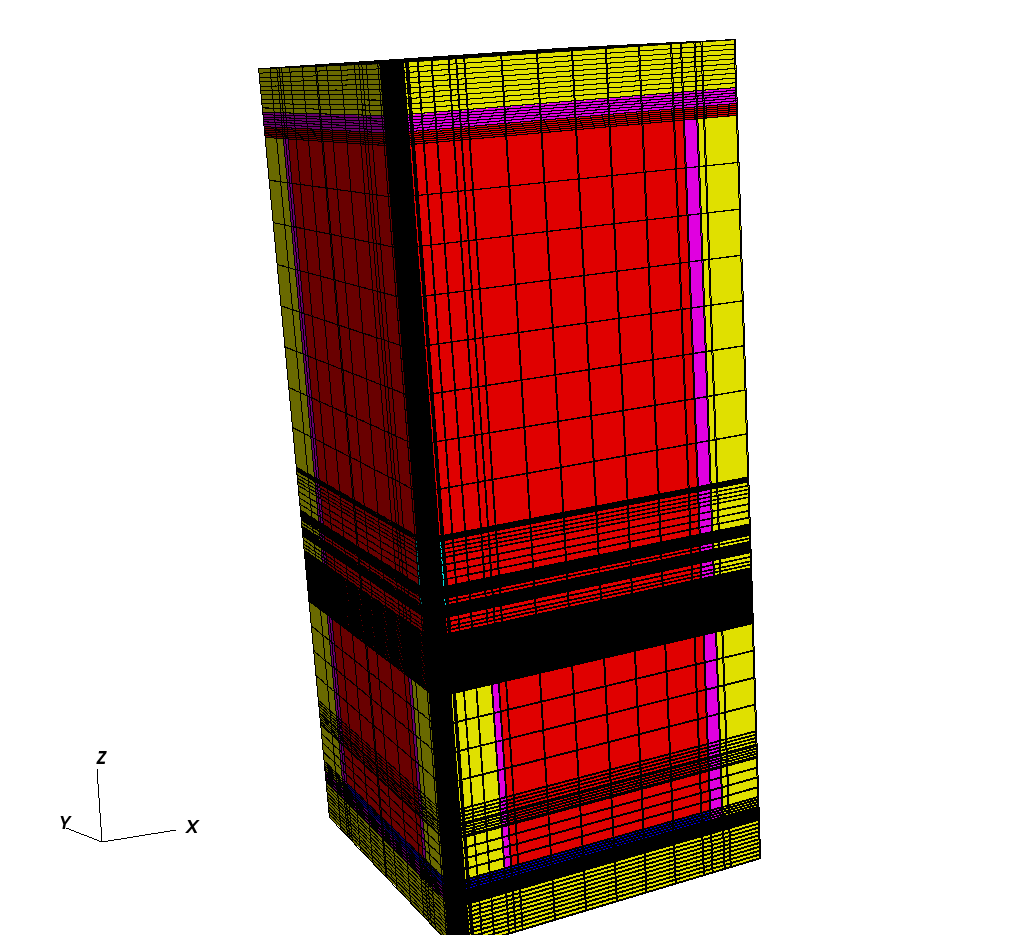
\includegraphics[scale=0.17]{../figures/im1c_prism.png}
\caption{A comparison of the two meshing approaches for the IM1C experiment.}
\label{comparison}
\end{figure}

\begin{figure}[H]
\centering
  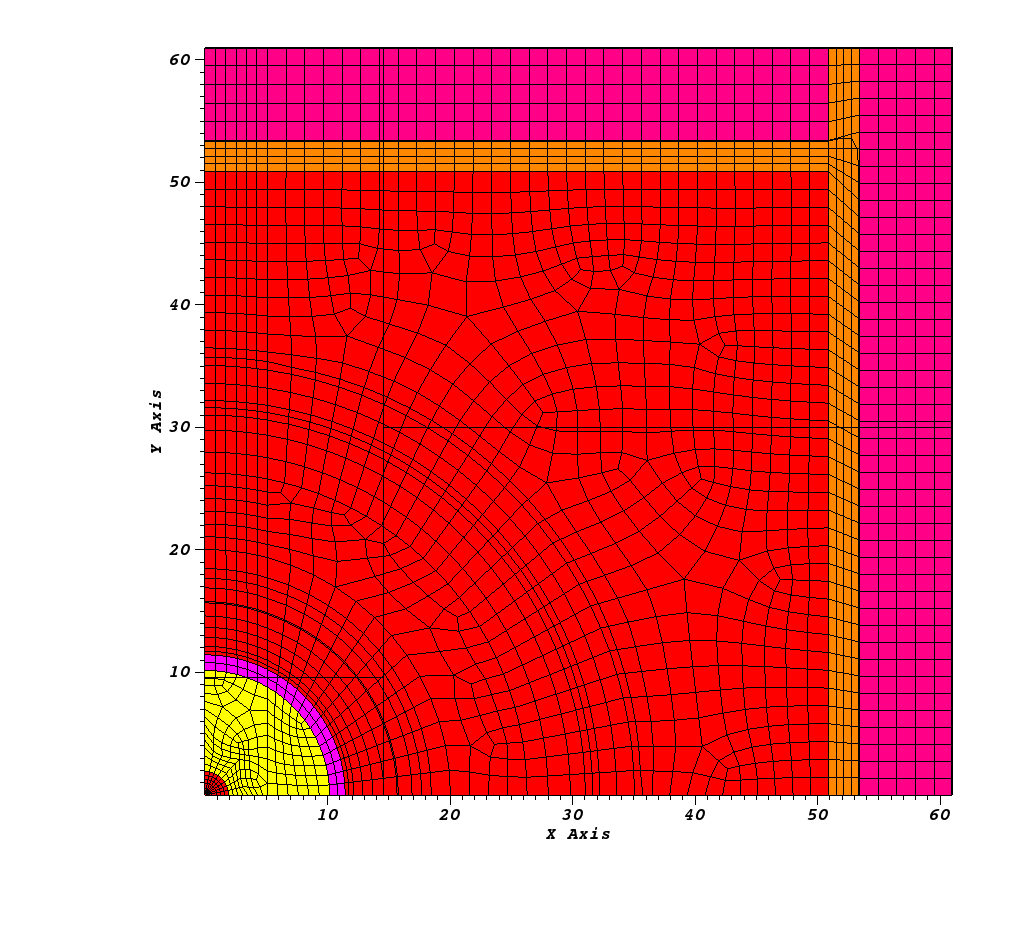
\includegraphics[scale=0.17]{../figures/im1_cubit_slice.png}
  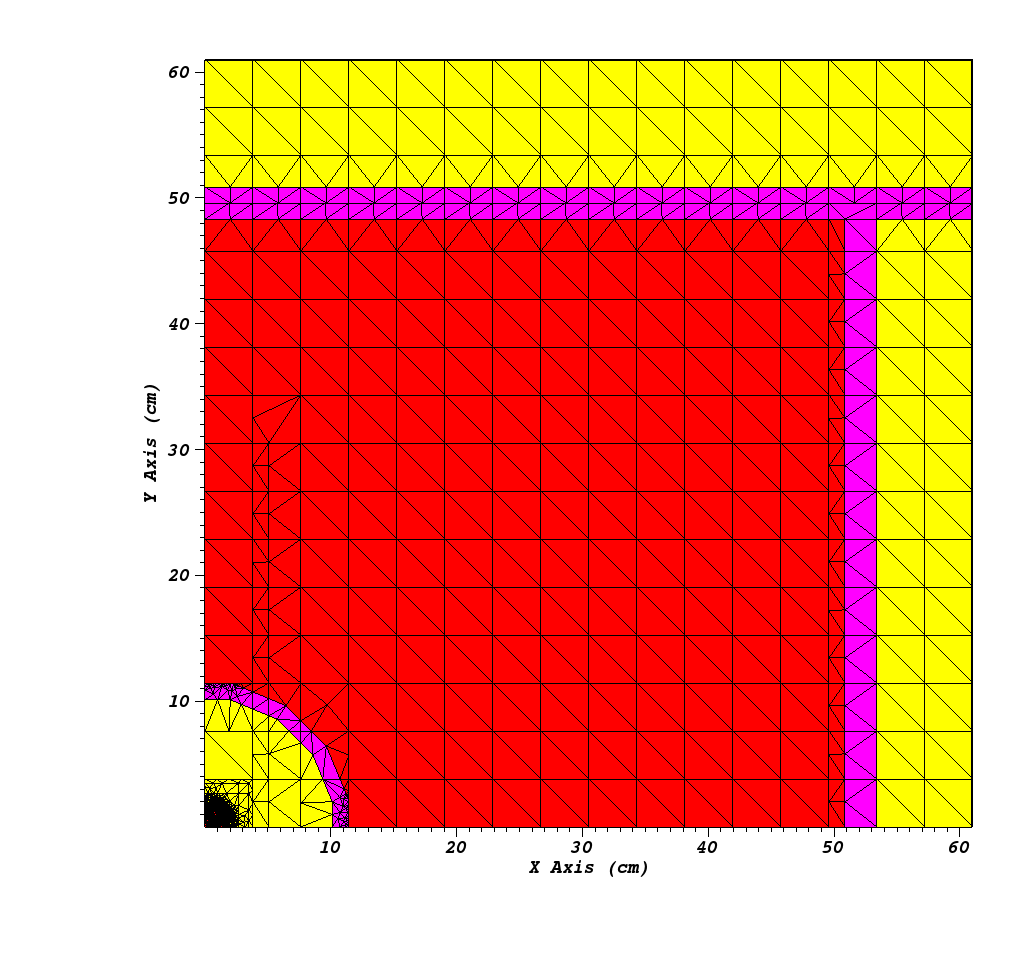
\includegraphics[scale=0.17]{../figures/im1c_prism_slice_q.png}
  \caption{A comparison of the two meshing approaches for a slice into the detector of the IM1C experiment.}
  \label{comparison_slice}
\end{figure}

\begin{figure}[H]
\centering
  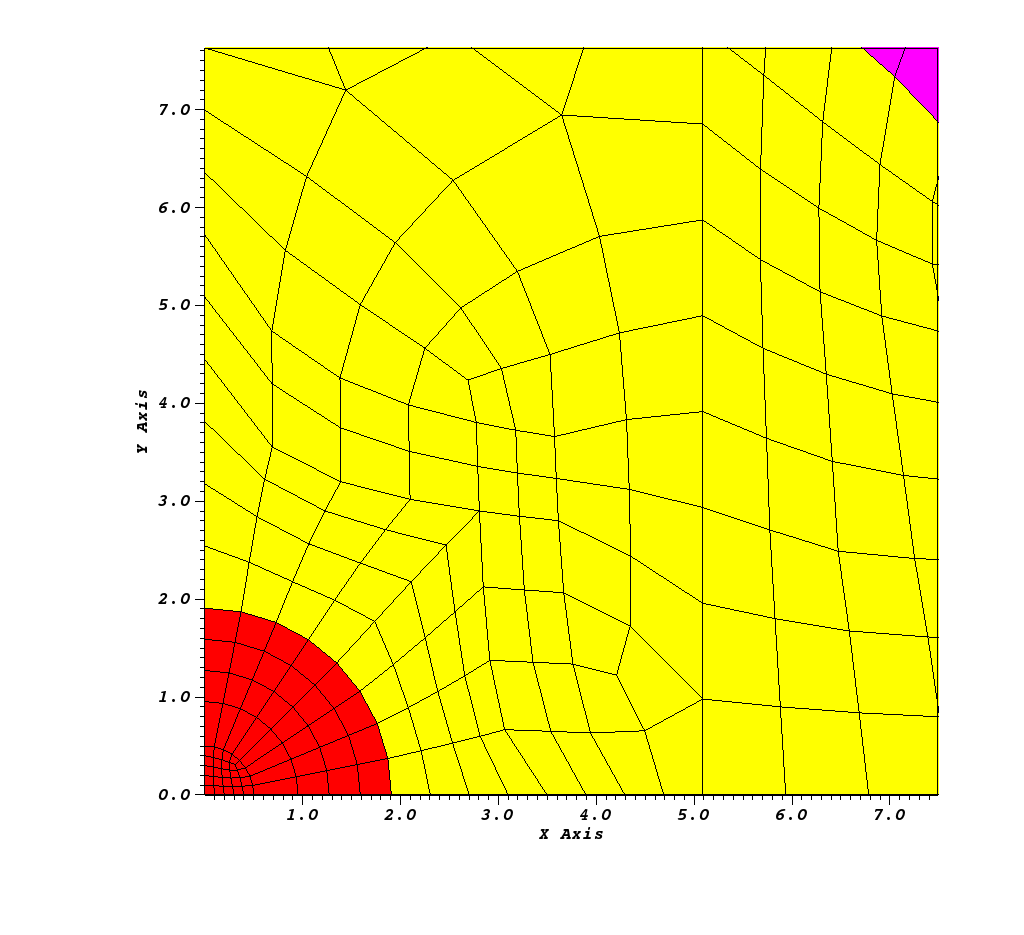
\includegraphics[scale=0.17]{../figures/im1_cubit_slice_zoom.png}
  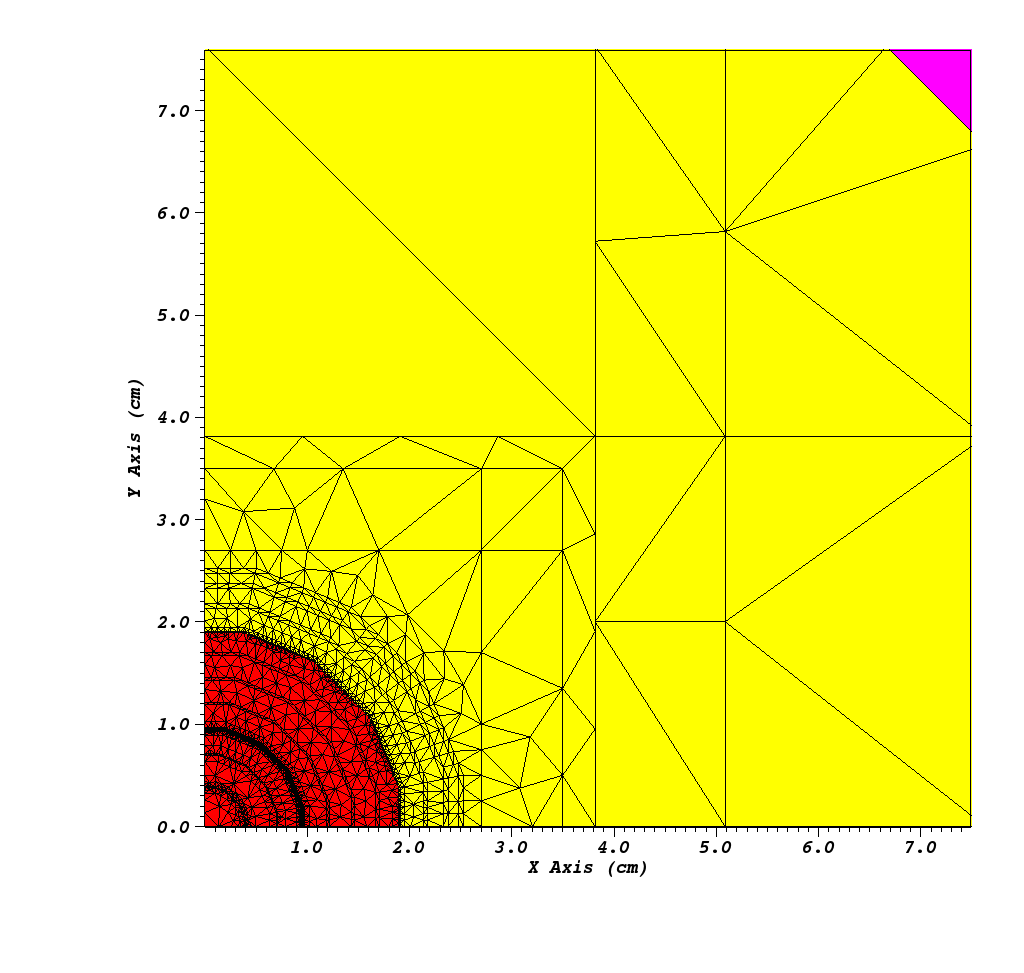
\includegraphics[scale=0.17]{../figures/im1c_prism_slice_zoom_q.png}
  \caption{A closer look at the detector region of the two meshing approaches.}
  \label{comparison_slice_zoom}
\end{figure}

As shown in Fig. \ref{comparison_slice_zoom}, the other advantage of the OpenFOAM meshes is the ability to maintain good mesh quality with a relatively smaller number of cells. Due to the extrusion process in the triangular prism meshes, any spherical or cylindrical shapes are stair-stepped in 2D, and need a lot more triangular cells to maintain a good mesh quality.

However, the OpenFOAM meshes due pose a challenge. When aggregating angles during the sweep, cycles occur. This prevents PDT from sweeping on these meshes unless using single angle aggregation, and most sweeps on large problems time out. A sweep structure that detects and addresses cycles is currently being implemented by the PDT development team, making OpenFOAM meshes practical for realistic problems.

\section{Issue and Approaches of Load Balancing on Unstructured Meshes}

When discussing the parallel scaling of transport sweeps, a load balanced problem is of great importance. A load balanced problem has an equal number of degrees of freedom per processor. Load balancing is important in order to minimize idle time for all processors by equally distributing (as much as possible) the work each processor has to do.  For the purposes of unstructured meshes in PDT, we are looking to ``balance'' the number of cells. Ideally, each processor will be responsible for an equal number of cells. 

If the number of cells in each subset can be reasonably balanced, then the problem is effectively load balanced. The Load Balance algorithm described below details how the subsets will be load balanced. In summary, the procedure of the algorithm involves moving the initially user specified $x$ and $y$ cut planes, re-meshing, and iterating until a reasonably load balanced problem is obtained. 

\noindent\begin{minipage}{\textwidth}
\textbf{Load Balance:} A load balancing algorithm that equalizes the number of triangles per subset. \\
\rule{\textwidth}{0.4pt}
\begin{algorithmic}
\STATE  $I,J$ subsets specified by user

\STATE Mesh all subsets

\STATE  $N_{tot} = $ total number of triangles
\STATE  $N_{ij} = $ number of triangles in subset $ij$

\STATE $f =\underset{ij}{\text{max}}(N_{ij})/\frac{N_{tot}}{I\cdot J}$

\COMMENT {//Check if all subsets meet the tolerance}
\IF {$f < \text{tol}_{\text{subset}}$}
	\STATE DONE with load balancing
\ELSE
	\STATE $f_I = \underset{i}{\text{max}}[\sum_{j} N_{ij}]/\frac{N_{tot}}{I}$
	
	\STATE $f_J = \underset{j}{\text{max}}[\sum_{i} N_{ij}]/\frac{N_{tot}}{J}$
	
	\IF {$f_I > \text{tol}_{\text{row}}$}
		\STATE \textbf{Redistribute}($X_i$)
	\ENDIF
	
	\IF{$f_J > \text{tol}_{\text{col}}$}
		\STATE \textbf{Redistribute}($Y_j$)
	\ENDIF 
	
	\IF {redistribution occured}
		\STATE REMESH and repeat algorithm
	\ENDIF
	
\ENDIF

\IF {There is still a discrepancy amongst subsets}
     \STATE Move cutplane segments on the subset level and remesh (may require changes to scheduling algorithm)
\ENDIF
\end{algorithmic}
\rule{\textwidth}{0.4pt}
\end{minipage}

\bigskip

\noindent\begin{minipage}{\textwidth}
\textbf{Redistribute:} A function that moves cut lines in either X or Y. \\
\rule{\textwidth}{0.4pt}
\begin{algorithmic}
\STATE \textbf{Input:}CutLines (X or Y vector that stores cut lines). 
\STATE \textbf{Input:} num\_tri\_row or num\_tri\_col, a pArray containing number of triangles in each row or column 
\STATE \textbf{Input:} The total number of triangles in the domain, $N_{tot}$

\STATE stapl::array\_view num\_tri\_view, over num\_tri\_row/column
\STATE stapl::array\_vew offset\_view

\STATE stapl::partial\_sum(num\_tri\_view) \COMMENT {Perform prefix sum}

\COMMENT {We now have a cumulative distribution stored in offset\_view}

\FOR {$i = 1$ :CutLines.size()-1}

	\STATE vector $<$double$>$ pt1 = [CutLines(i-1), offset\_view(i-1)]
	\STATE vector $<$double$>$ pt2 = [CutLines(i), offset\_view(i)]
	\STATE ideal\_value = $i\cdot \frac{N_{tot}}{\text{CutLines.size()}-1}$
	\STATE X-intersect(pt1,pt2,ideal\_value) \COMMENT{Calculates the X-intersect of the line formed by pt1 and pt2 and the line y = ideal\_value.}
	\STATE CutLines(i) = X-intersect
\ENDFOR
\end{algorithmic}
\rule{\textwidth}{0.4pt}
\end{minipage}

\subsection{Load Balancing by Dimension} \label{lbd_section}

In previous work, load balancing proved to be successful, but not as successful as initially expected. It became clear that when creating an unstructured mesh in PDT, the iterative nature of our algorithm did not work as effectively when using the Triangle Mesh Generator. 

An improved load balancing algorithm was implemented that significantly improved our metric. Rather than load balancing both dimensions within an iteration, one dimension is balanced first for all iterations, and then the cut lines that yielded the best metric for that dimension are chosen. Then the next dimension is balanced within the first dimension. For example, if the $x$ cut lines are balanced first, the $y$ cut lines would be balanced \textit{within} each column. When full 3D load balancing by dimension (shown in Fig. \ref{lbd} is used via Rick Vega's code, excellent metrics within 5\% of unity are consistently obtained.

\begin{figure}[H]
\centering
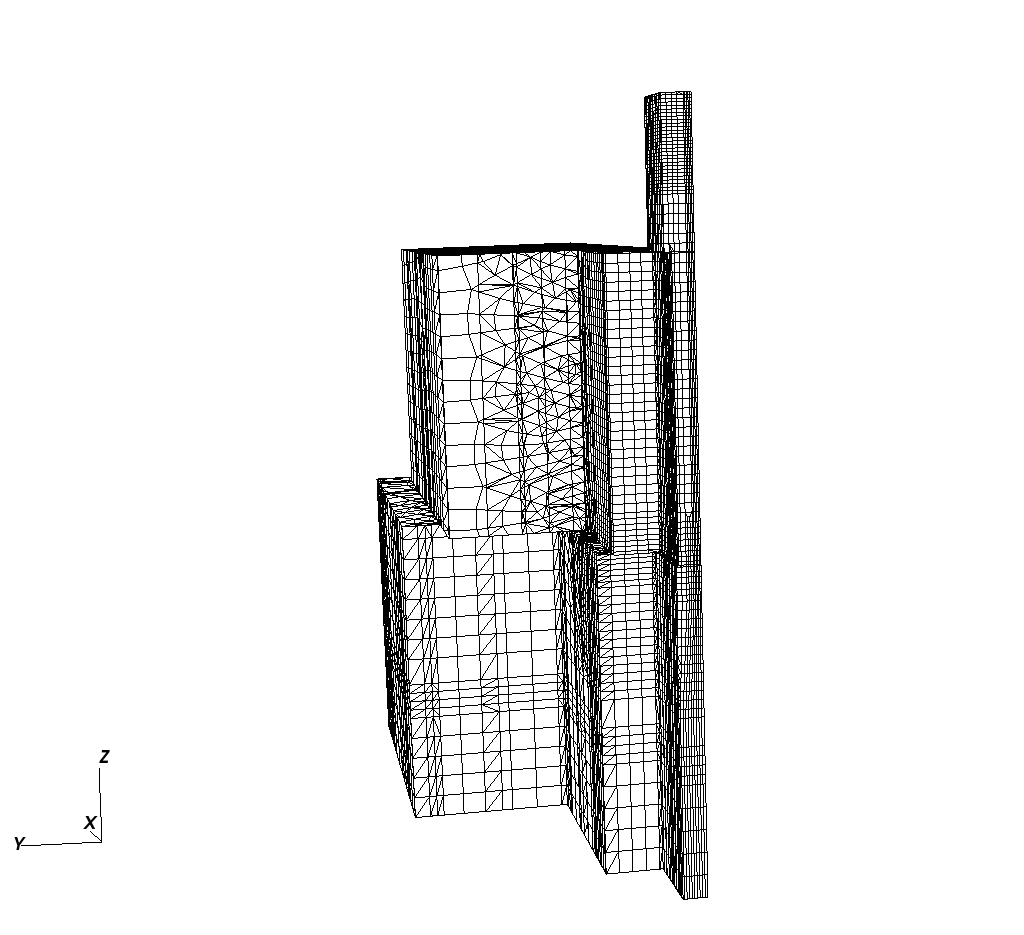
\includegraphics[scale=0.5]{../figures/im1_foam_448.png}
\caption{A slice of the IM1C experiment showcasing load balancing by dimension in 3D with an OpenFOAM mesh.}
\label{lbd}
\end{figure}

Upon further study of the load balancing by dimension algorithm, it is clear the most efficient partitioning scheme is not being used. A cost function that takes into account the best partitioning scheme and best balance needs to be studied. The best balanced partition may not be the best partition for a parallel transport sweep.


\section{Drawbacks of Load Balancing Unstructured Meshes for Transport Sweeps}

While perfect load balance was the initial goal, we need to know how this affects the efficiency of our parallel transport sweep. Figures \ref{regular_partition}-\ref{worst_partition} showcase the theoretical effect of perfect load balance on the transport sweep.

Figure \ref{regular_partition} shows a sweep domain with a regular partition with perfect balance (equivalent number of cells per processor). The sweep maintains a mostly regular wavelike structure as each angle sweeps through the domain, and this sweep completes in 40 stages. This is the ideal partitioning for the transport sweep, but often hard to achieve with unstructured meshes \textbf{and} perfect balance.

\begin{figure}[H]
  \centering
  \begin{subfigure}{0.49\textwidth}
  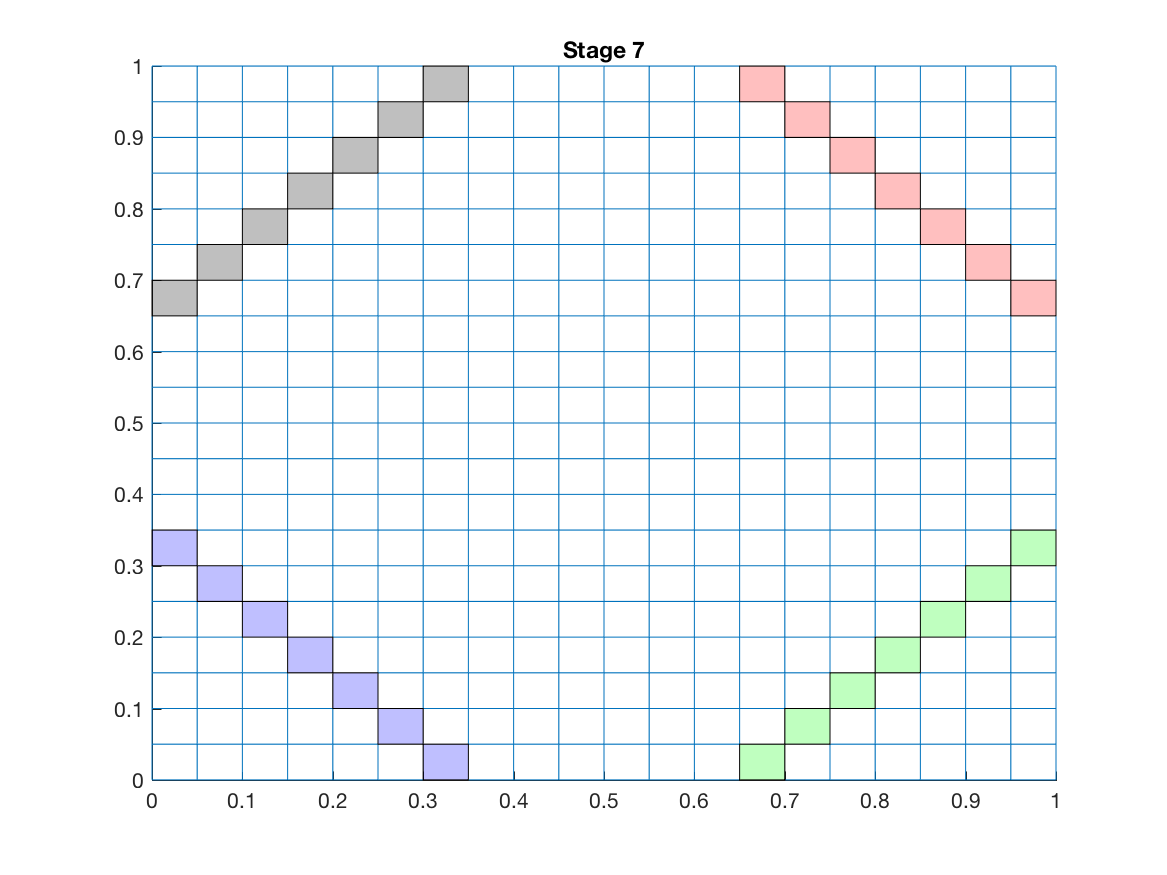
\includegraphics[scale=0.5]{../figures/regular_partition_1.png}
  \end{subfigure}
  \begin{subfigure}{0.49\textwidth}
  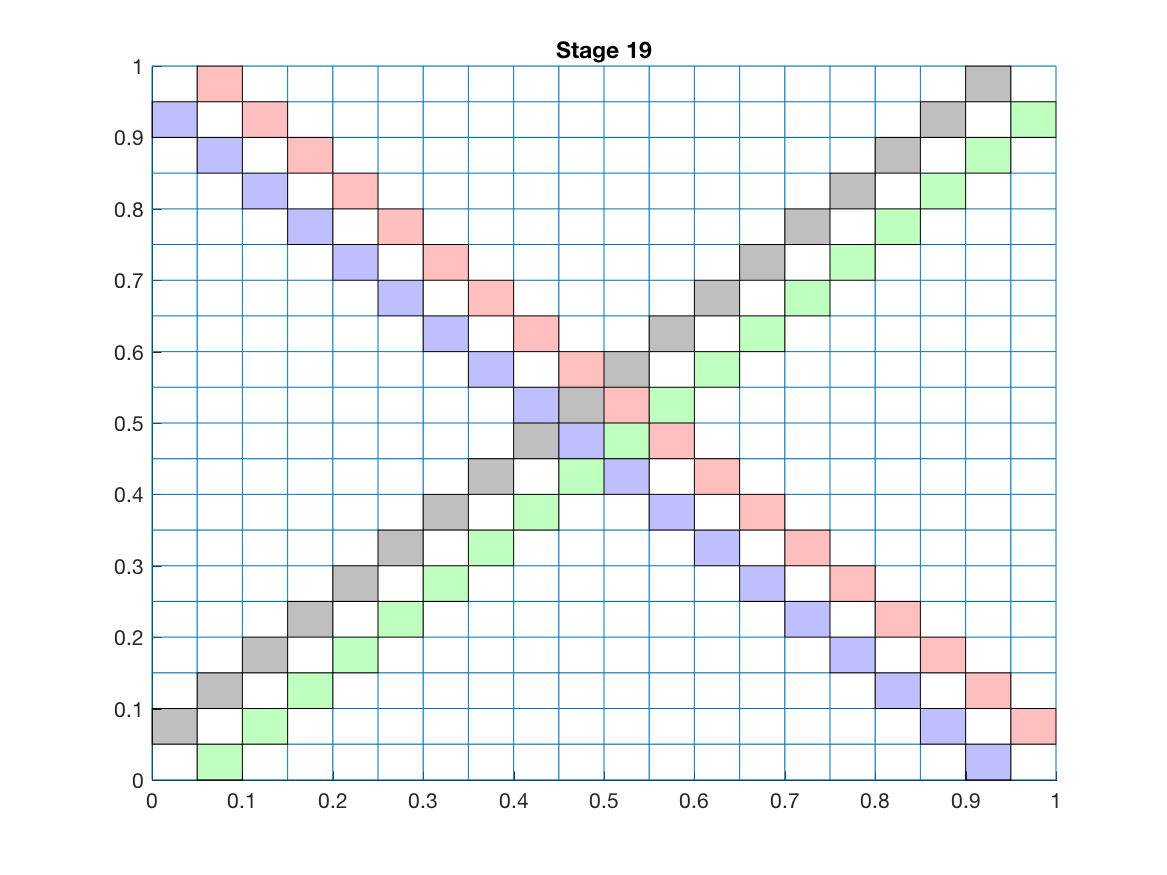
\includegraphics[scale=0.5]{../figures/regular_partition_2.png}
  \end{subfigure}
  \begin{subfigure}{0.49\textwidth}
  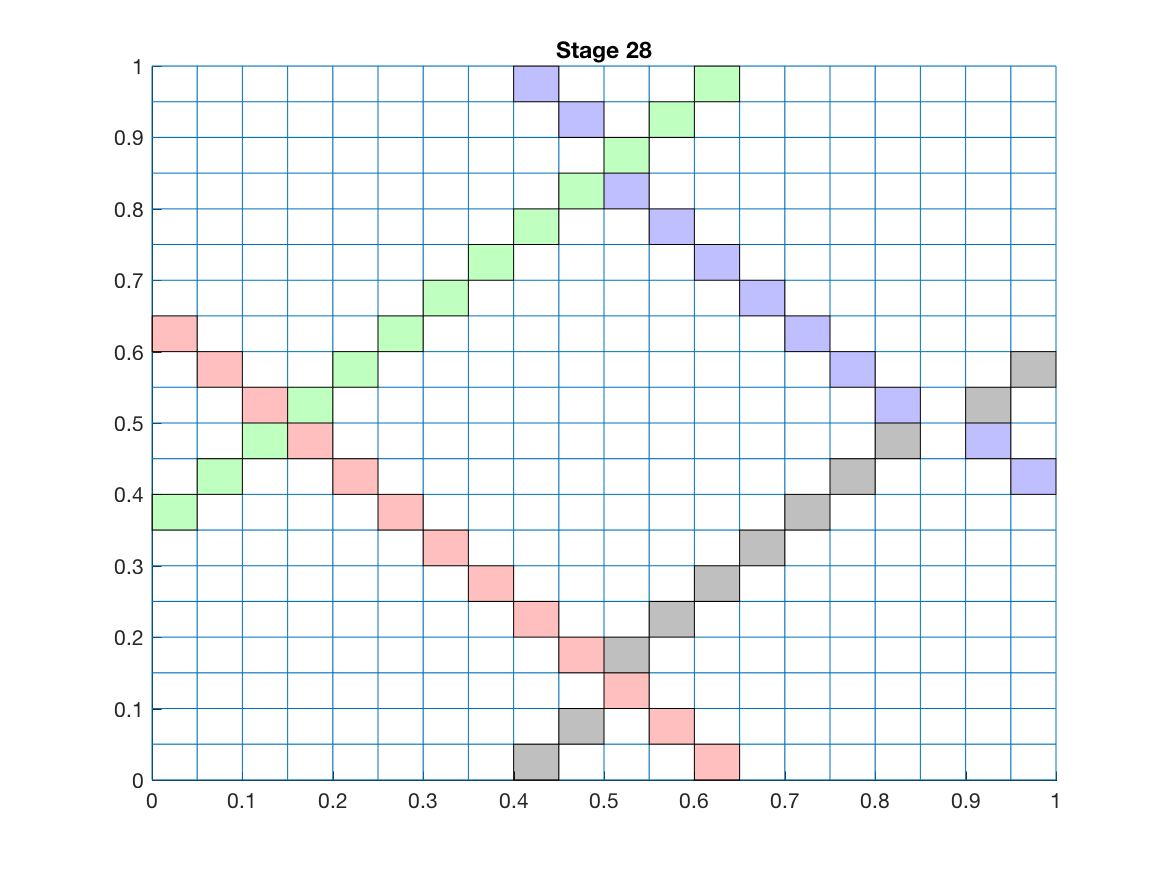
\includegraphics[scale=0.5]{../figures/regular_partition_3.png}
  \end{subfigure}
  \begin{subfigure}{0.49\textwidth}
  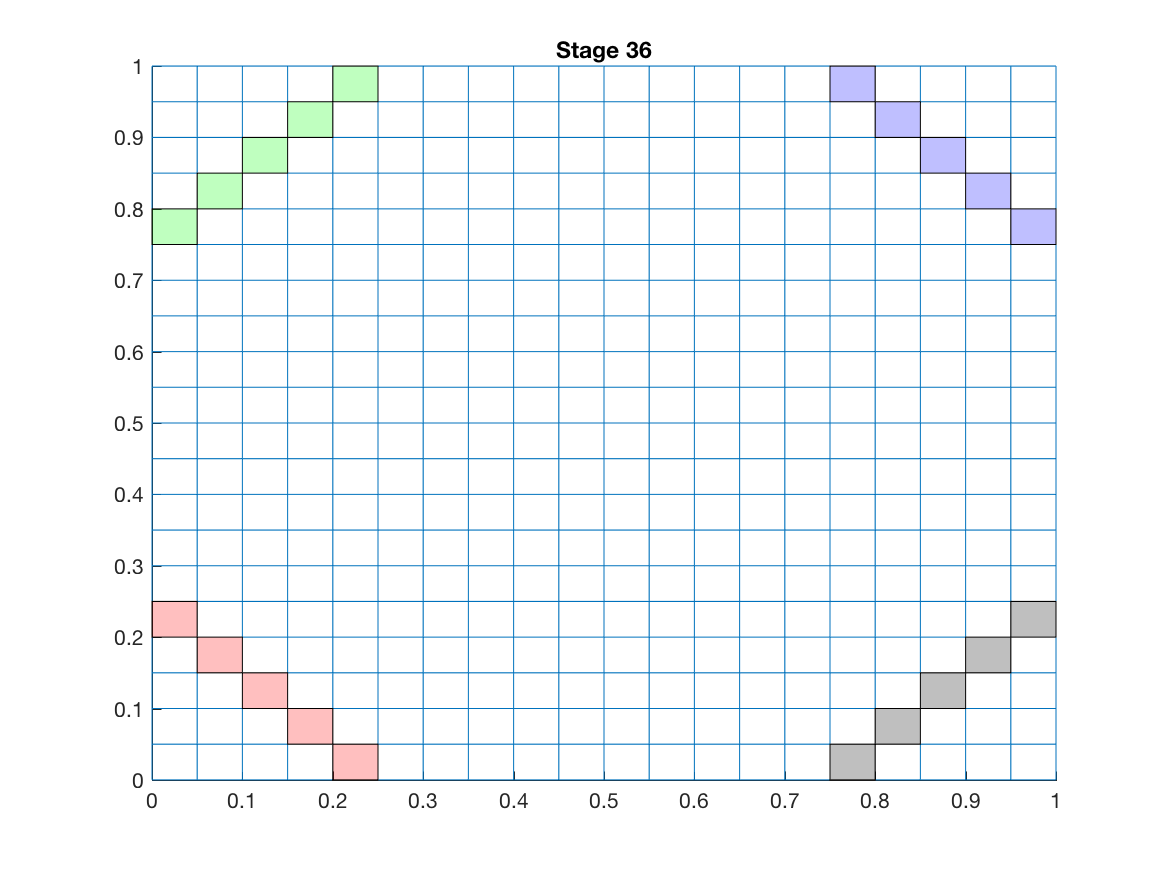
\includegraphics[scale=0.5]{../figures/regular_partition_4.png}
  \end{subfigure}
  \caption{The transport sweep using a regular partition with perfect balance.}
  \label{regular_partition}
\end{figure}

With the improved load balancing by dimension, we are likely to see a partition similar to the partitioning shown in Fig. \ref{random_partition} for all geometries. It is immediately observable that we don't have the same wavelike transport sweep, as communication penalties take their toll. As a result, this sweep completes in 101 stages, as opposed to 40 stages for the regular partition.


\begin{figure}[H]
  \centering
  \begin{subfigure}{0.49\textwidth}
  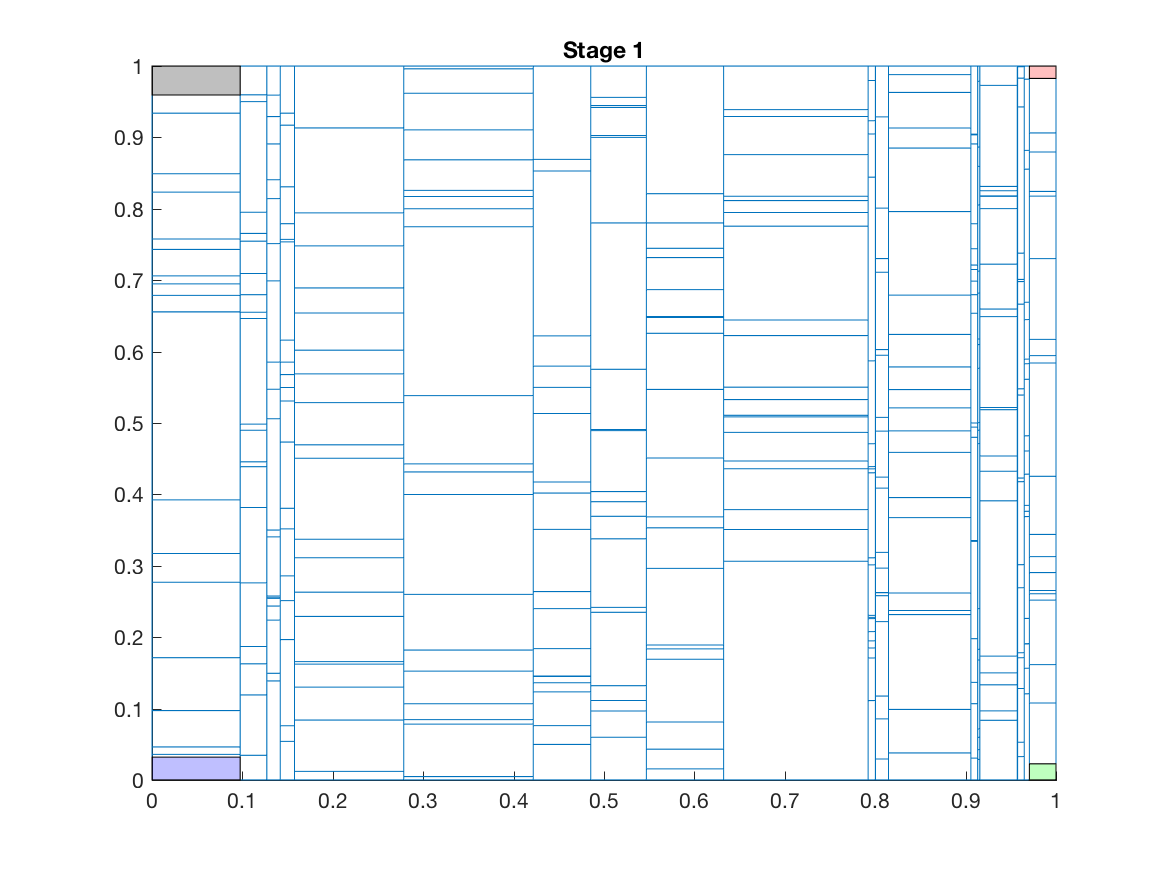
\includegraphics[scale=0.5]{../figures/random_partition_1.png}
  \end{subfigure}
  \begin{subfigure}{0.49\textwidth}
  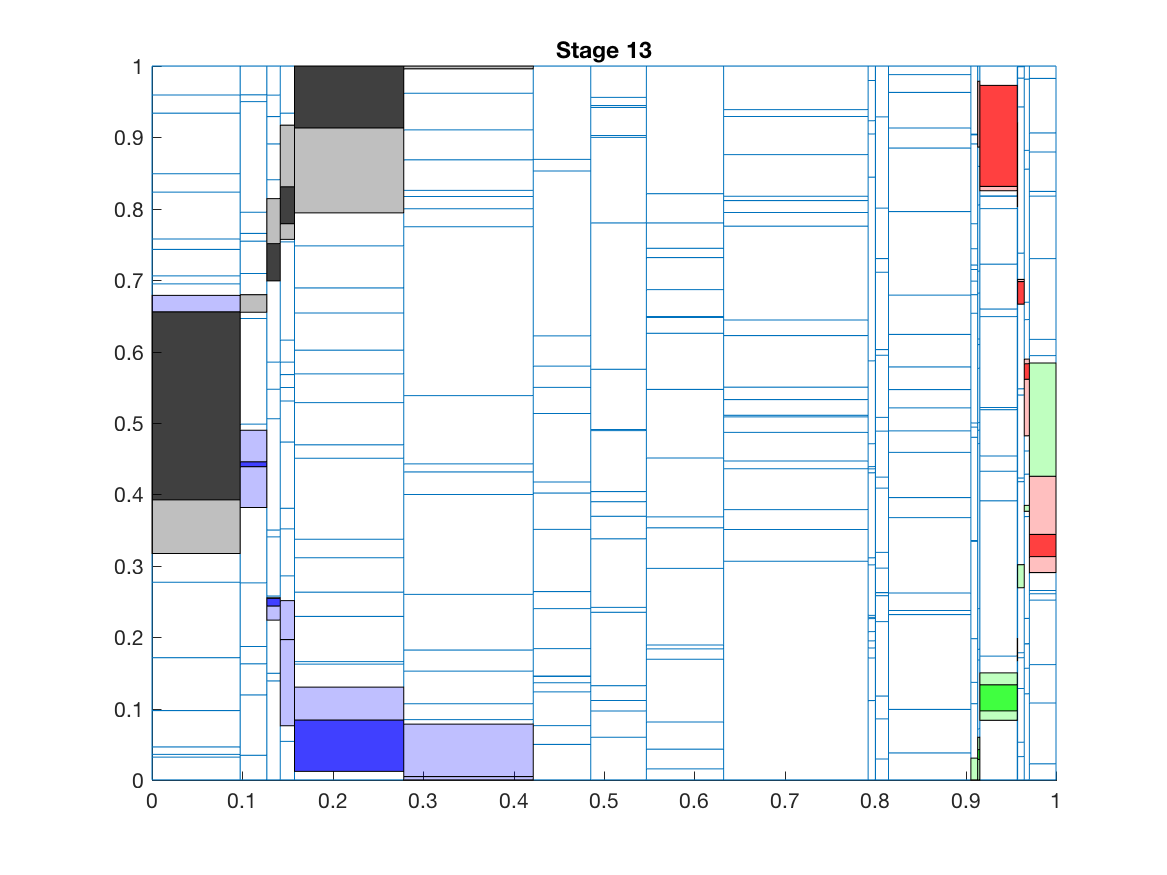
\includegraphics[scale=0.5]{../figures/random_partition_2.png}
  \end{subfigure}
  \begin{subfigure}{0.49\textwidth}
  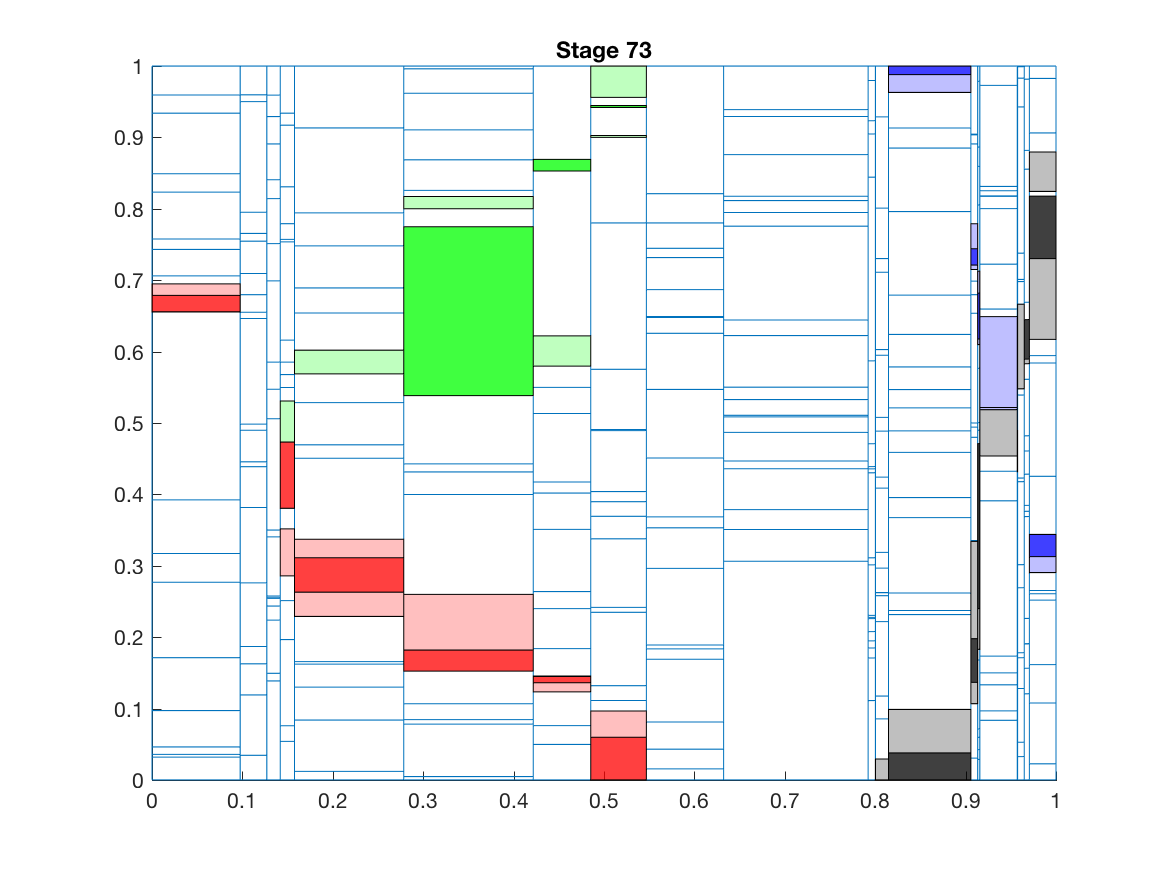
\includegraphics[scale=0.5]{../figures/random_partition_3.png}
  \end{subfigure}
  \begin{subfigure}{0.49\textwidth}
  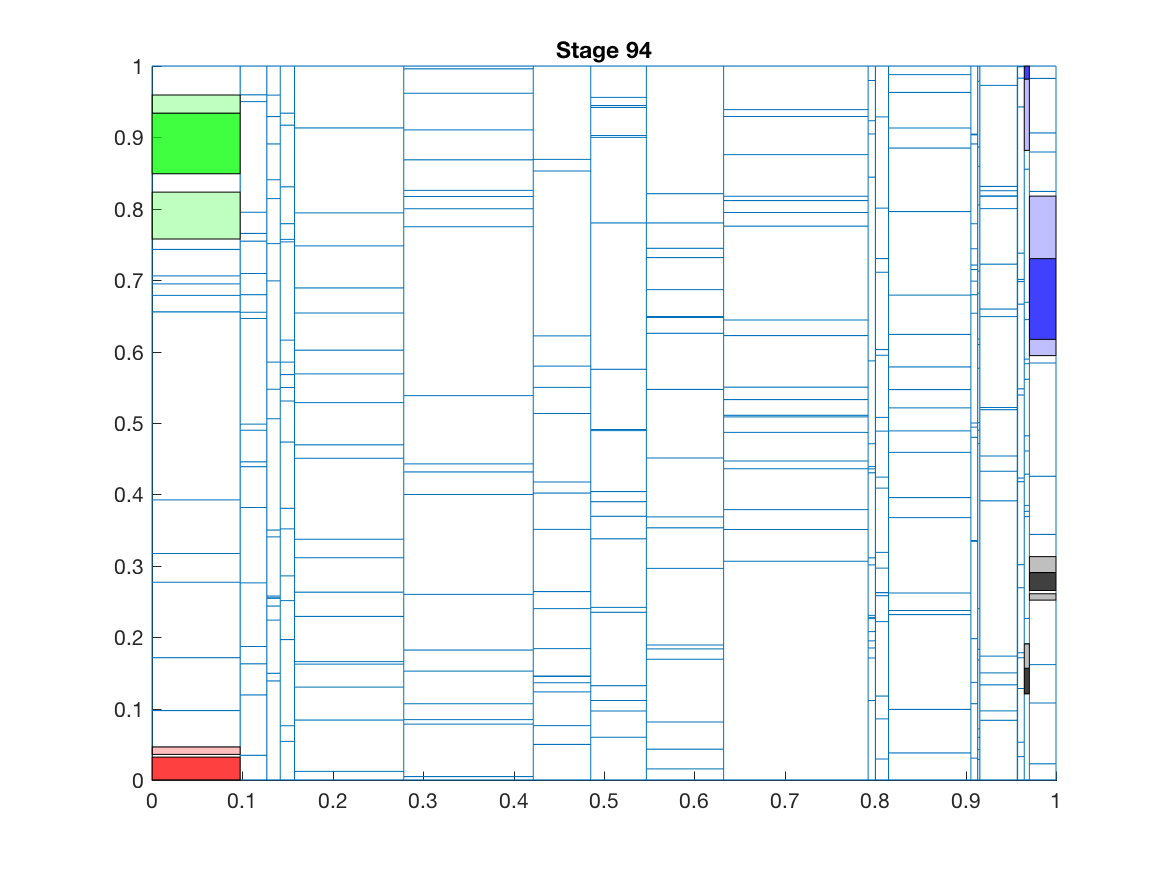
\includegraphics[scale=0.5]{../figures/random_partition_4.png}
  \end{subfigure}
  \caption{The transport sweep using a random partition with perfect balance.}
  \label{random_partition}
\end{figure}

Figure \ref{worst_partition} observes the worst theoretical sweep partitioning, where the transport sweep takes on a snake-like behavior. This partitioning yields a stage count of 230, which is far worse than even the random partitioning stage count of 101.

\begin{figure}[H]
  \centering
  \begin{subfigure}{0.49\textwidth}
  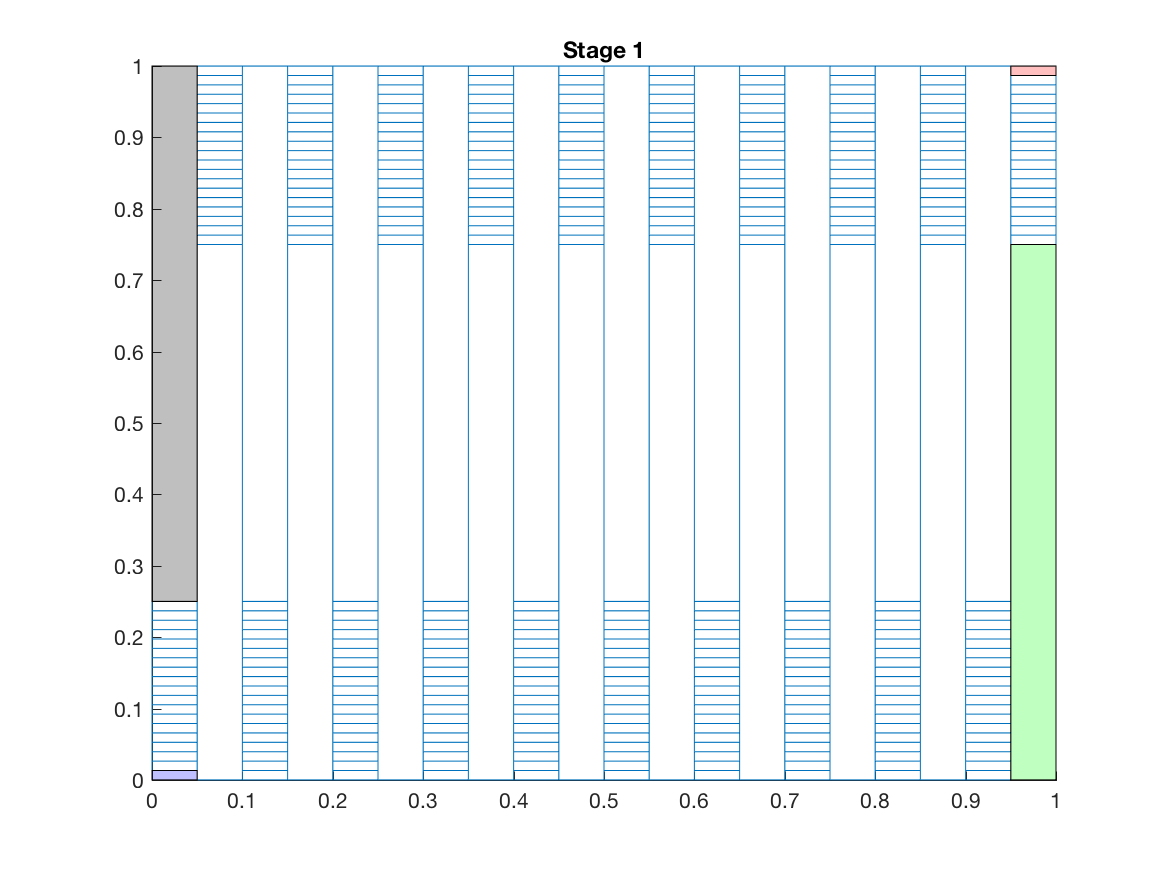
\includegraphics[scale=0.5]{../figures/worst_partition_1.png}
  \end{subfigure}
  \begin{subfigure}{0.49\textwidth}
  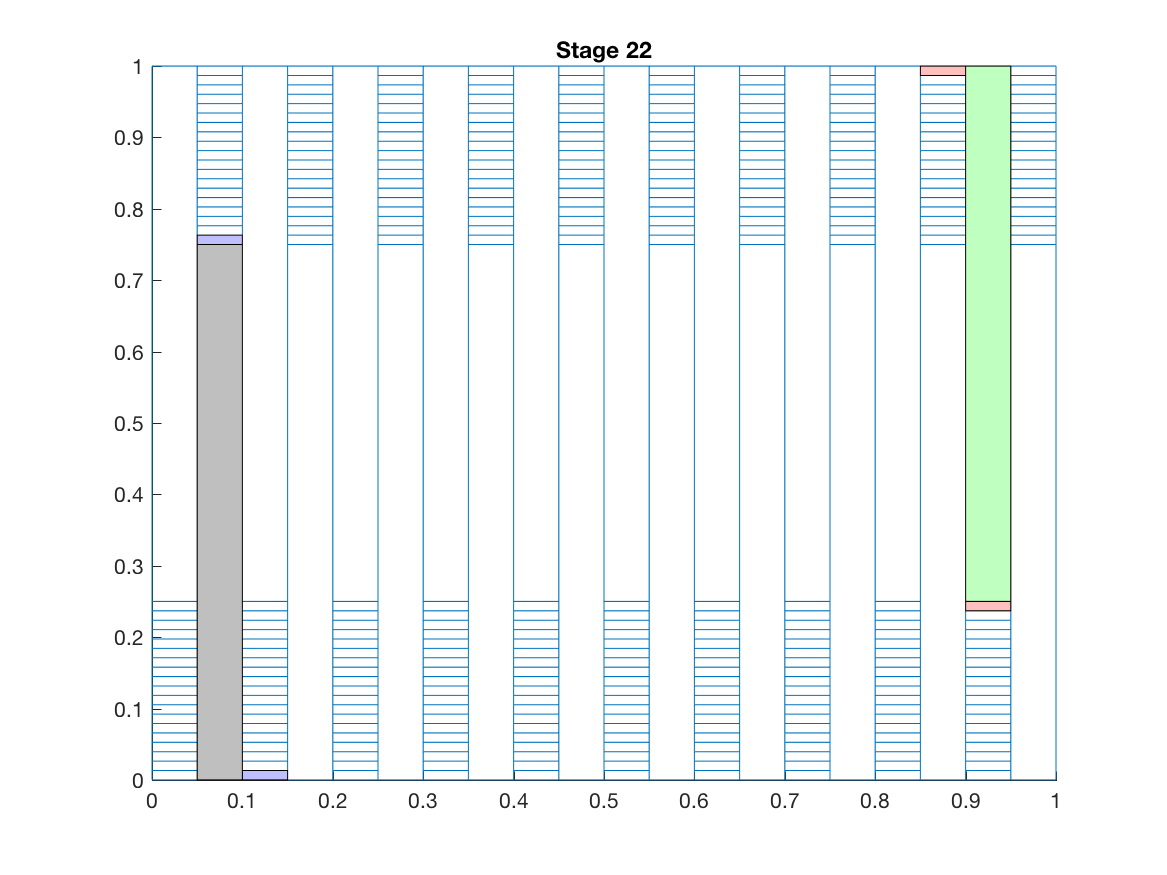
\includegraphics[scale=0.5]{../figures/worst_partition_2.png}
  \end{subfigure}
  \begin{subfigure}{0.49\textwidth}
  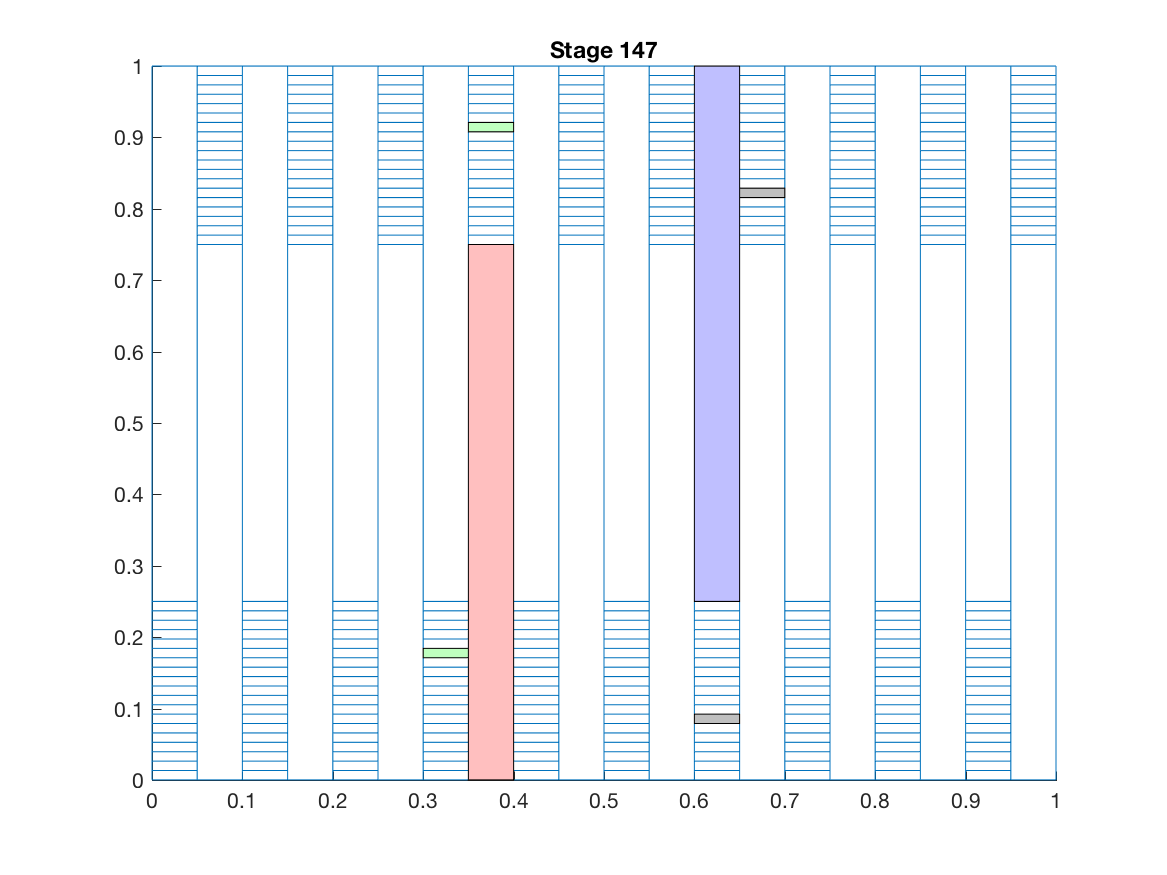
\includegraphics[scale=0.5]{../figures/worst_partition_3.png}
  \end{subfigure}
  \begin{subfigure}{0.49\textwidth}
  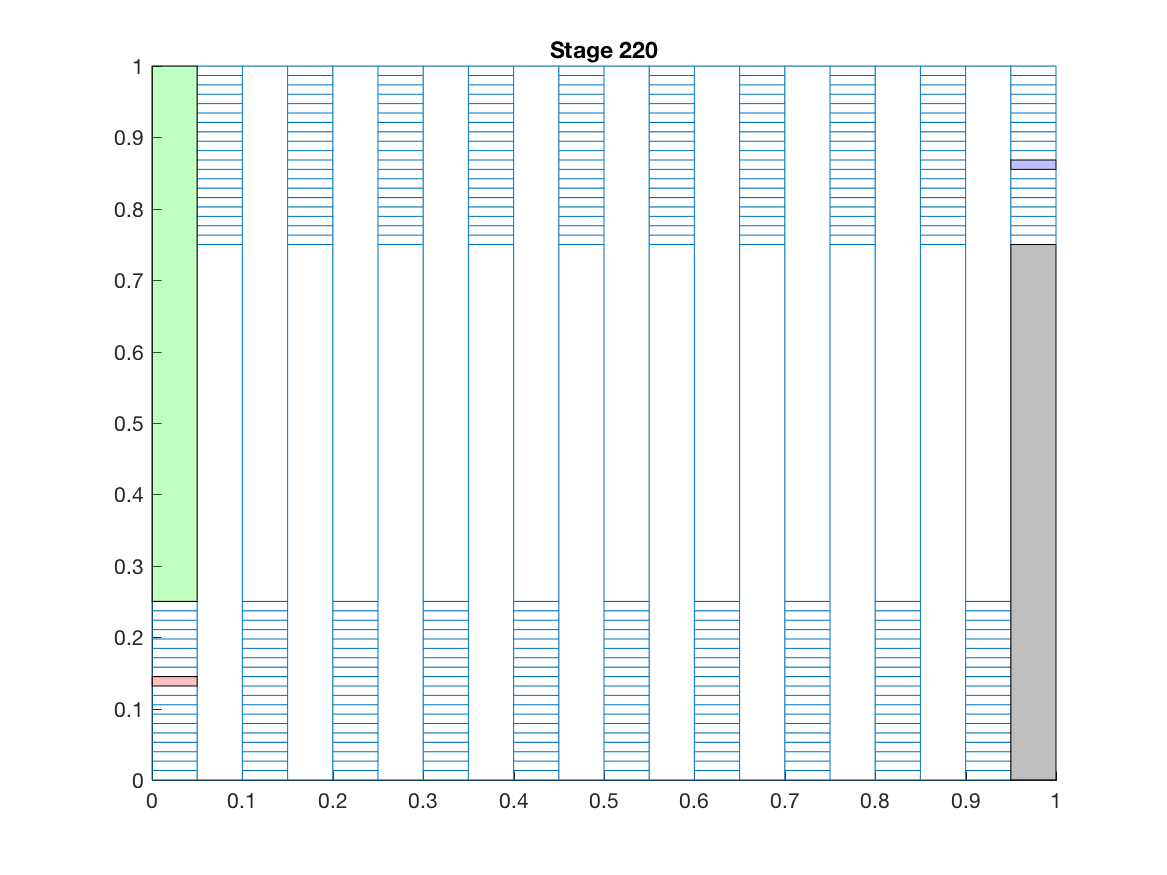
\includegraphics[scale=0.5]{../figures/worst_partition_4.png}
  \end{subfigure}
  \caption{The transport sweep using the worst partition with perfect balance.}
  \label{worst_partition}
\end{figure}

Two things become immediately clear as a result of this study: perfect balance does not always yield the best parallel efficiency, and the stage count of a sweep is no longer as important. The concept of the stage is invalidated, because a stage relies on the assumption of perfect load balance. Once the time to compute a task changes throughout the problem domain, we must instead rely on the total time to solution as the most important metric, not the stage and the previously staged definition of parallel efficiency (Eq. \ref{paralleleff}). 

\section{Time to Solution Estimation} \label{TOS}

In order to optimize the location of the cut lines based on balance and sweep efficiency without relying on a costly iterative process, we must build a time to solution estimator. For a given partition, this tool will estimate the time to solution. This is done by building directed task dependence graphs for each octant (quadrant in 2D) and weighting the graph edges based on certain criteria discussed Section \ref{weighting_graphs} Figure \ref{subset_plot} shows an example subset partitioning scheme in 3D, and the corresponding task dependence graph (TDG) for the front bottom octant is shown in Fig. \ref{digraph}.

\begin{figure}[H]
\centering
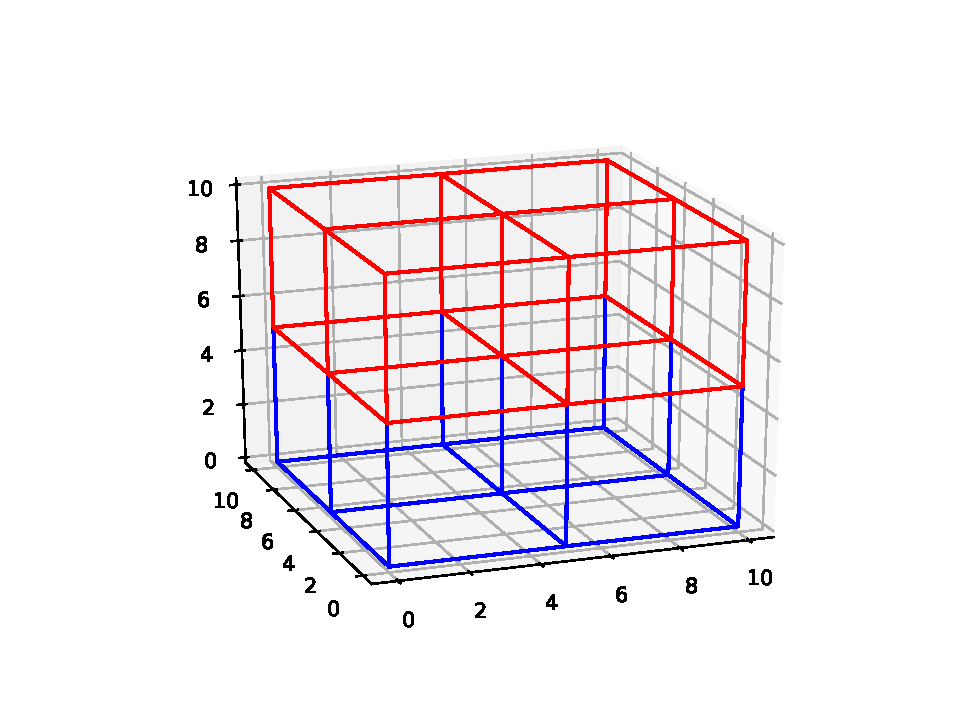
\includegraphics{../figures/subset_plot.pdf}
\caption{An example uniform partitioning scheme.}
\label{subset_plot}
\end{figure}

\begin{figure}[H]
\centering
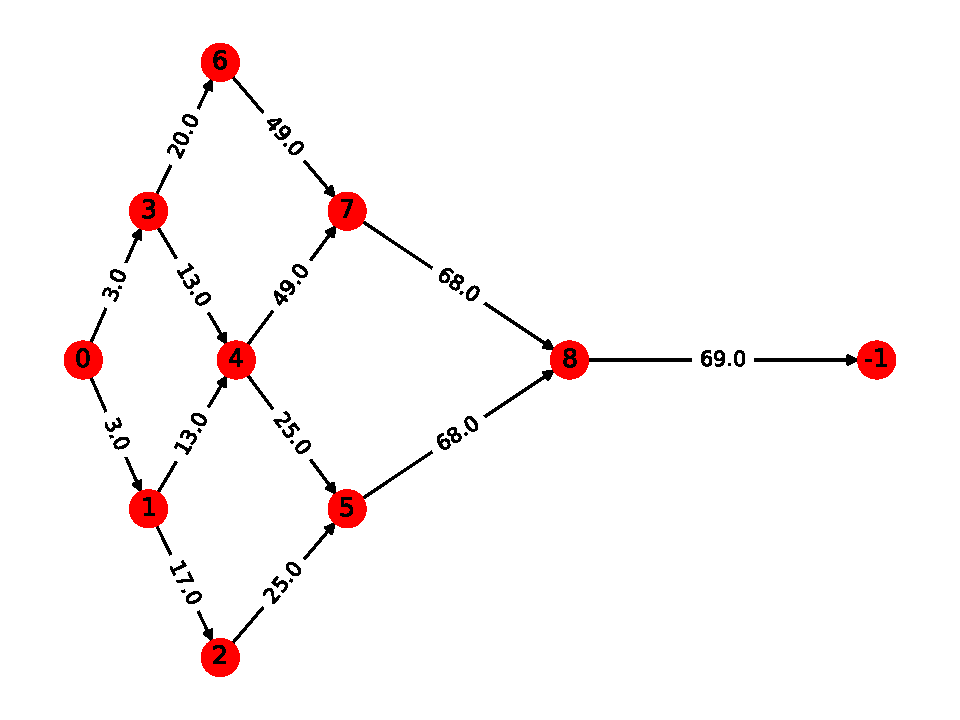
\includegraphics{../figures/digraph.pdf}
\caption{The task dependence graph for the front bottom octant in Fig. \ref{subset_plot} with weights assigned.}
\label{digraph}
\end{figure}

\subsection{Weighting the Task Dependence Graph}\label{weighting_graphs}

The time to solution relies on weighting the graph correctly to determine the traversal time for each octant. In order to correctly estimate the time to solution, two pieces of information are initially required: the number of cells per subset, and the number of boundary cells per subset. In order to obtain this information, a very fine grid is superimposed upon the domain partitioning, with each grid unit containing $g$ cells. Equation \eqref{num_mini_sub} gives the total number of fine grid units $n_s$, and Eqns. \eqref{boundaries_begin} - \eqref{boundaries} give $a,b, \text{and }  c$, the global domain boundaries in each dimension. 
%Equations.
\begin{align}
\label{num_mini_sub}
n_s &= \frac{\text{number of cells}}{g} \\
\label{boundaries_begin}
a &= x_{\text{max}} - x_{\text{min}} \\
b &= y_{\text{max}} - y_{\text{min}} \\
c &= z_{\text{max}} - z_{\text{min}} 
\label{boundaries}
\end{align}
%Text
Equations \eqref{num_x} - \eqref{num_z} calculate the number of fine grid units in each direction.
%Equations
\begin{align}
\label{num_x}
n_{x} &= a \cdot \Big(\frac{n_s}{a\cdot b \cdot c}\Big)^{1/3} \\
n_{y} &= b \cdot \Big(\frac{n_s}{a\cdot b \cdot c}\Big)^{1/3} \\
n_{z} &= c \cdot \Big(\frac{n_s}{a\cdot b \cdot c}\Big)^{1/3} 
\label{num_z}
\end{align}

Combining $n_x, n_y, \text{and } n_z$ with the cut line information in each direction allows us to compute the fine grid units in each subset and along each boundary.  

Given that we know the machine parameters (grind time, latency, message communication time), Eq. \ref{cost_calculation} estimates how long it takes to solve and communicate all unknowns in a given subset:

\begin{equation}
\text{cost} = N_s\cdot T_g + N_b\cdot T_{\text{comm}} + \text{latency}\cdot M_l,
\label{cost_calculation}
\end{equation}
%end eq
where $N_u$ is the number of unknowns in the subset, $T_g$ is the grind time, $N_b$ is the number of unknowns along the subset boundaries, $T_\text{comm}$ is the communication time per unknown, and $M_l$ is the machine dependent latency multiplier. 

The cost value is used to help appropriately weight the edges in each TDG independently. We weight the TDGs according to the following algorithm:

\begin{algorithm}[H]
\begin{algorithmic}
\FOR{$node = 1$ to $N$}
\STATE Weight outgoing edges with the cost of solving and communicating $node$.
\ENDFOR
\FOR{$node = 1$ to $N$}
\STATE Find longest path to $node$
\STATE Set all incoming edge weights to $node$ to the sum of the longest path to the node.
\ENDFOR
\label{universalweights}
\end{algorithmic}
\end{algorithm}

This algorithm effectively sets up the initial weights in each TDG to represent a crucial piece of information: the time at which each node is ready to solve. In other words, all incoming weights to a node will share the same value, which represents the time that node is ready to solve factoring in upstream dependencies. 

\subsubsection{Conflict Detection and Resolution}

Once this is done for all edges in all TDGs, we have to detect and address sweep conflicts between all the TDGs. We do so with the following algorithm:
\begin{algorithm}[H]
\begin{algorithmic}
\STATE t = 0
\WHILE{num\_finished\_graphs $<$ num\_graphs}
\STATE{Get nodes that are being solved at time t}
\STATE{Find conflicting graphs in nodes being solved}
\IF{No conflicting graphs in nodes being solved}
	\STATE{t = time of next interaction}
\ELSE
	\STATE{Find first conflicted node}
	\STATE{Get conflicting graphs at first conflicted node}
	\STATE{Modify graph weights according to which graph wins the conflict}
	\IF{Number of conflicted nodes is 1}
	\STATE{t = time of next interaction}
	\ENDIF
\ENDIF
\STATE{Check how many graphs have finished by time t}
\ENDWHILE
\label{conflict}
\end{algorithmic}
\end{algorithm}

This algorithm marches along all TDGs and at every time $t$ that a node is reached, checks for conflicts and modifies downstream weights accordingly. 

Two forms of conflict resolution are being explored, depth-of-graph remaining and first come first serve. Due to the imbalanced nature of the problems, each subset will take a different amount of time to solve and communicate, defaulting conflict resolution to a first come first basis. If two graphs reach a node at the same time, then the graph with the greater depth-of-graph remaining wins. If there is still a tie, then the graph with the priority octant wins.

\subsection{Optimizing the Time to Solution}\label{optimize}

Once the heaviest paths of each TDG are weighted appropriately with conflicts taken into account, we simply take the final weight of the ending node as the time to solution for that graph. The octant with the heaviest sweep time is used as the time to solution for a given partitioning scheme. We will use a python optimization tool in order to get the best partitioning scheme possible. The cut lines will be the input parameter, and the tool will iterate on this parameter to minimize the time to solution. 

\section{Goals and Proposed Plan}

\begin{itemize}
\item Devise and implement a load balancing by dimension algorithm in PDT (Section \ref{lbd_section}).
\item Devise and implement a time-to-solution estimator that returns the maximum time to solution for a given partitioning scheme (Section \ref{TOS}).
\item Verify time-to-solution estimator matches PDT's sweep time with equivalent aggregation parameters and scheduling.
\item Use time-to-solution estimator to optimize cut line locations by using it as a cost function in a Python optimization library (scipy.minimize, scipy.optimize, etc.). 
\item Build test problems, in 2D and 3D, that balance approximately perfectly via both load balancing algorithms.
\item Using these test problems, show that optimizing partitions with the proposed approach yields a better runtime.
\item Implement these tests in PDT and show that the optimized partitions yield a better runtime than perfectly load balanced problems.
\item Explore adding the threads per processor as a variable to our parameter space during optimization in addition to cut lines.
\end{itemize}


\bibliographystyle{plain}
\bibliography{./Proposal}

\end{document}
